\documentclass[twoside]{book}

% Packages required by doxygen
\usepackage{fixltx2e}
\usepackage{calc}
\usepackage{doxygen}
\usepackage[export]{adjustbox} % also loads graphicx
\usepackage{graphicx}
\usepackage[utf8]{inputenc}
\usepackage{makeidx}
\usepackage{multicol}
\usepackage{multirow}
\PassOptionsToPackage{warn}{textcomp}
\usepackage{textcomp}
\usepackage[nointegrals]{wasysym}
\usepackage[table]{xcolor}

% Font selection
\usepackage[T1]{fontenc}
\usepackage[scaled=.90]{helvet}
\usepackage{courier}
\usepackage{amssymb}
\usepackage{sectsty}
\renewcommand{\familydefault}{\sfdefault}
\allsectionsfont{%
  \fontseries{bc}\selectfont%
  \color{darkgray}%
}
\renewcommand{\DoxyLabelFont}{%
  \fontseries{bc}\selectfont%
  \color{darkgray}%
}
\newcommand{\+}{\discretionary{\mbox{\scriptsize$\hookleftarrow$}}{}{}}

% Page & text layout
\usepackage{geometry}
\geometry{%
  a4paper,%
  top=2.5cm,%
  bottom=2.5cm,%
  left=2.5cm,%
  right=2.5cm%
}
\tolerance=750
\hfuzz=15pt
\hbadness=750
\setlength{\emergencystretch}{15pt}
\setlength{\parindent}{0cm}
\setlength{\parskip}{0.2cm}
\makeatletter
\renewcommand{\paragraph}{%
  \@startsection{paragraph}{4}{0ex}{-1.0ex}{1.0ex}{%
    \normalfont\normalsize\bfseries\SS@parafont%
  }%
}
\renewcommand{\subparagraph}{%
  \@startsection{subparagraph}{5}{0ex}{-1.0ex}{1.0ex}{%
    \normalfont\normalsize\bfseries\SS@subparafont%
  }%
}
\makeatother

% Headers & footers
\usepackage{fancyhdr}
\pagestyle{fancyplain}
\fancyhead[LE]{\fancyplain{}{\bfseries\thepage}}
\fancyhead[CE]{\fancyplain{}{}}
\fancyhead[RE]{\fancyplain{}{\bfseries\leftmark}}
\fancyhead[LO]{\fancyplain{}{\bfseries\rightmark}}
\fancyhead[CO]{\fancyplain{}{}}
\fancyhead[RO]{\fancyplain{}{\bfseries\thepage}}
\fancyfoot[LE]{\fancyplain{}{}}
\fancyfoot[CE]{\fancyplain{}{}}
\fancyfoot[RE]{\fancyplain{}{\bfseries\scriptsize Generated on Tue Mar 3 2015 15\+:23\+:19 for Points by Doxygen }}
\fancyfoot[LO]{\fancyplain{}{\bfseries\scriptsize Generated on Tue Mar 3 2015 15\+:23\+:19 for Points by Doxygen }}
\fancyfoot[CO]{\fancyplain{}{}}
\fancyfoot[RO]{\fancyplain{}{}}
\renewcommand{\footrulewidth}{0.4pt}
\renewcommand{\chaptermark}[1]{%
  \markboth{#1}{}%
}
\renewcommand{\sectionmark}[1]{%
  \markright{\thesection\ #1}%
}

% Indices & bibliography
\usepackage{natbib}
\usepackage[titles]{tocloft}
\setcounter{tocdepth}{3}
\setcounter{secnumdepth}{5}
\makeindex

% Hyperlinks (required, but should be loaded last)
\usepackage{ifpdf}
\ifpdf
  \usepackage[pdftex,pagebackref=true]{hyperref}
\else
  \usepackage[ps2pdf,pagebackref=true]{hyperref}
\fi
\hypersetup{%
  colorlinks=true,%
  linkcolor=blue,%
  citecolor=blue,%
  unicode%
}

% Custom commands
\newcommand{\clearemptydoublepage}{%
  \newpage{\pagestyle{empty}\cleardoublepage}%
}


%===== C O N T E N T S =====

\begin{document}

% Titlepage & ToC
\hypersetup{pageanchor=false,
             bookmarks=true,
             bookmarksnumbered=true,
             pdfencoding=unicode
            }
\pagenumbering{roman}
\begin{titlepage}
\vspace*{7cm}
\begin{center}%
{\Large Points }\\
\vspace*{1cm}
{\large Generated by Doxygen 1.8.9.1}\\
\vspace*{0.5cm}
{\small Tue Mar 3 2015 15:23:19}\\
\end{center}
\end{titlepage}
\clearemptydoublepage
\tableofcontents
\clearemptydoublepage
\pagenumbering{arabic}
\hypersetup{pageanchor=true}

%--- Begin generated contents ---
\chapter{Hierarchical Index}
\section{Class Hierarchy}
This inheritance list is sorted roughly, but not completely, alphabetically\+:\begin{DoxyCompactList}
\item \contentsline{section}{array$<$ T $>$}{\pageref{classarray}}{}
\item \contentsline{section}{Boundary}{\pageref{class_boundary}}{}
\item \contentsline{section}{Grid\+Points}{\pageref{class_grid_points}}{}
\item \contentsline{section}{Point}{\pageref{class_point}}{}
\begin{DoxyCompactList}
\item \contentsline{section}{Domain}{\pageref{class_domain}}{}
\end{DoxyCompactList}
\item \contentsline{section}{Sparse\+\_\+\+Matrix}{\pageref{class_sparse___matrix}}{}
\item \contentsline{section}{Vector$<$ T $>$}{\pageref{class_vector}}{}
\end{DoxyCompactList}

\chapter{Class Index}
\section{Class List}
Here are the classes, structs, unions and interfaces with brief descriptions\+:\begin{DoxyCompactList}
\item\contentsline{section}{\hyperlink{class_compute_matrix}{Compute\+Matrix} \\*This class computes the matrix for the poison process }{\pageref{class_compute_matrix}}{}
\item\contentsline{section}{\hyperlink{class_iterative___solver}{Iterative\+\_\+\+Solver} \\*This class solves the linear equation A\+X = B }{\pageref{class_iterative___solver}}{}
\item\contentsline{section}{\hyperlink{class_sparse_matrix}{Sparse\+Matrix} \\*This class stores the value of matrix in sparse form }{\pageref{class_sparse_matrix}}{}
\item\contentsline{section}{\hyperlink{class_vector}{Vector$<$ T $>$} }{\pageref{class_vector}}{}
\end{DoxyCompactList}

\chapter{File Index}
\section{File List}
Here is a list of all files with brief descriptions\+:\begin{DoxyCompactList}
\item\contentsline{section}{src/\hyperlink{array_8h}{array.\+h} }{\pageref{array_8h}}{}
\item\contentsline{section}{src/\hyperlink{_boundary_8cpp}{Boundary.\+cpp} }{\pageref{_boundary_8cpp}}{}
\item\contentsline{section}{src/\hyperlink{_boundary_8h}{Boundary.\+h} }{\pageref{_boundary_8h}}{}
\item\contentsline{section}{src/\hyperlink{_domain_8cpp}{Domain.\+cpp} }{\pageref{_domain_8cpp}}{}
\item\contentsline{section}{src/\hyperlink{_domain_8h}{Domain.\+h} }{\pageref{_domain_8h}}{}
\item\contentsline{section}{src/\hyperlink{_grid_points_8cpp}{Grid\+Points.\+cpp} }{\pageref{_grid_points_8cpp}}{}
\item\contentsline{section}{src/\hyperlink{_grid_points_8h}{Grid\+Points.\+h} }{\pageref{_grid_points_8h}}{}
\item\contentsline{section}{src/\hyperlink{main_8cpp}{main.\+cpp} }{\pageref{main_8cpp}}{}
\item\contentsline{section}{src/\hyperlink{main__point_8cpp}{main\+\_\+point.\+cpp} }{\pageref{main__point_8cpp}}{}
\item\contentsline{section}{src/\hyperlink{_point_8cpp}{Point.\+cpp} }{\pageref{_point_8cpp}}{}
\item\contentsline{section}{src/\hyperlink{_point_8h}{Point.\+h} }{\pageref{_point_8h}}{}
\item\contentsline{section}{src/\hyperlink{_sparse_matrix_8cpp}{Sparse\+Matrix.\+cpp} }{\pageref{_sparse_matrix_8cpp}}{}
\item\contentsline{section}{src/\hyperlink{_sparse_matrix_8h}{Sparse\+Matrix.\+h} }{\pageref{_sparse_matrix_8h}}{}
\item\contentsline{section}{src/\hyperlink{_vector_8h}{Vector.\+h} }{\pageref{_vector_8h}}{}
\end{DoxyCompactList}

\chapter{Class Documentation}
\hypertarget{classarray}{}\section{array$<$ T $>$ Class Template Reference}
\label{classarray}\index{array$<$ T $>$@{array$<$ T $>$}}


{\ttfamily \#include $<$array.\+h$>$}

\subsection*{Public Member Functions}
\begin{DoxyCompactItemize}
\item 
\hyperlink{classarray_a090e68e6f659a8c24a3046d3b57617f7}{array} (int m, int n)
\item 
\hyperlink{classarray_a5a5249a0715f8e7e5422fb66f0f663f8}{$\sim$array} ()
\item 
void \hyperlink{classarray_ac6ac82ef5fecc273bd8f2d67b449c5ed}{display} ()
\item 
void \hyperlink{classarray_a010a4dd12776af094c33b8ae107c0ee9}{read\+\_\+values} ()
\item 
\hyperlink{classarray}{array} \hyperlink{classarray_ac0bd5fcf5f53194e14159f1a26b578f6}{operator+} (\hyperlink{classarray}{array})
\item 
\hyperlink{classarray}{array} \hyperlink{classarray_a521b6f90168c5c949ba5d814aee981ed}{operator-\/} (\hyperlink{classarray}{array})
\item 
\hyperlink{classarray}{array} \hyperlink{classarray_aafcac5ad6b36e4a93323f0d757aab02e}{operator$\ast$} (\hyperlink{classarray}{array})
\item 
\hyperlink{classarray}{array} \hyperlink{classarray_a57199cc30628af328c2d7f72b0c7b3b1}{add} (\hyperlink{classarray}{array})
\end{DoxyCompactItemize}
\subsection*{Private Member Functions}
\begin{DoxyCompactItemize}
\item 
void \hyperlink{classarray_a190f65c46755585269c87b065194aefd}{get\+Data} ()
\item 
void \hyperlink{classarray_afcc7d2bd10460a423cc2384bfc4d479f}{initialize} ()
\end{DoxyCompactItemize}
\subsection*{Private Attributes}
\begin{DoxyCompactItemize}
\item 
int \hyperlink{classarray_a7c38a7c022fd545cbb1d4ff62522a231}{row}
\item 
int \hyperlink{classarray_a0722d2ae3a709aa8abadac67a3c0b003}{column}
\item 
T $\ast$$\ast$ \hyperlink{classarray_acaddf8a3372a3910c35ee4e15bce513e}{A}
\end{DoxyCompactItemize}


\subsection{Constructor \& Destructor Documentation}
\hypertarget{classarray_a090e68e6f659a8c24a3046d3b57617f7}{}\index{array@{array}!array@{array}}
\index{array@{array}!array@{array}}
\subsubsection[{array}]{\setlength{\rightskip}{0pt plus 5cm}template$<$class T $>$ {\bf array}$<$ T $>$\+::{\bf array} (
\begin{DoxyParamCaption}
\item[{int}]{m, }
\item[{int}]{n}
\end{DoxyParamCaption}
)}\label{classarray_a090e68e6f659a8c24a3046d3b57617f7}
\hypertarget{classarray_a5a5249a0715f8e7e5422fb66f0f663f8}{}\index{array@{array}!````~array@{$\sim$array}}
\index{````~array@{$\sim$array}!array@{array}}
\subsubsection[{$\sim$array}]{\setlength{\rightskip}{0pt plus 5cm}template$<$class T $>$ {\bf array}$<$ T $>$\+::$\sim${\bf array}$<$ T $>$ (
\begin{DoxyParamCaption}
{}
\end{DoxyParamCaption}
)}\label{classarray_a5a5249a0715f8e7e5422fb66f0f663f8}


\subsection{Member Function Documentation}
\hypertarget{classarray_a57199cc30628af328c2d7f72b0c7b3b1}{}\index{array@{array}!add@{add}}
\index{add@{add}!array@{array}}
\subsubsection[{add}]{\setlength{\rightskip}{0pt plus 5cm}template$<$class T$>$ {\bf array} {\bf array}$<$ T $>$\+::add (
\begin{DoxyParamCaption}
\item[{{\bf array}$<$ T $>$}]{}
\end{DoxyParamCaption}
)}\label{classarray_a57199cc30628af328c2d7f72b0c7b3b1}
\hypertarget{classarray_ac6ac82ef5fecc273bd8f2d67b449c5ed}{}\index{array@{array}!display@{display}}
\index{display@{display}!array@{array}}
\subsubsection[{display}]{\setlength{\rightskip}{0pt plus 5cm}template$<$class T $>$ void {\bf array}$<$ T $>$\+::display (
\begin{DoxyParamCaption}
{}
\end{DoxyParamCaption}
)}\label{classarray_ac6ac82ef5fecc273bd8f2d67b449c5ed}
\hypertarget{classarray_a190f65c46755585269c87b065194aefd}{}\index{array@{array}!get\+Data@{get\+Data}}
\index{get\+Data@{get\+Data}!array@{array}}
\subsubsection[{get\+Data}]{\setlength{\rightskip}{0pt plus 5cm}template$<$class T $>$ void {\bf array}$<$ T $>$\+::get\+Data (
\begin{DoxyParamCaption}
{}
\end{DoxyParamCaption}
)\hspace{0.3cm}{\ttfamily [private]}}\label{classarray_a190f65c46755585269c87b065194aefd}
\hypertarget{classarray_afcc7d2bd10460a423cc2384bfc4d479f}{}\index{array@{array}!initialize@{initialize}}
\index{initialize@{initialize}!array@{array}}
\subsubsection[{initialize}]{\setlength{\rightskip}{0pt plus 5cm}template$<$class T $>$ void {\bf array}$<$ T $>$\+::initialize (
\begin{DoxyParamCaption}
{}
\end{DoxyParamCaption}
)\hspace{0.3cm}{\ttfamily [private]}}\label{classarray_afcc7d2bd10460a423cc2384bfc4d479f}
\hypertarget{classarray_aafcac5ad6b36e4a93323f0d757aab02e}{}\index{array@{array}!operator$\ast$@{operator$\ast$}}
\index{operator$\ast$@{operator$\ast$}!array@{array}}
\subsubsection[{operator$\ast$}]{\setlength{\rightskip}{0pt plus 5cm}template$<$class T $>$ {\bf array}$<$ T $>$ {\bf array}$<$ T $>$\+::operator$\ast$ (
\begin{DoxyParamCaption}
\item[{{\bf array}$<$ T $>$}]{matrix2}
\end{DoxyParamCaption}
)}\label{classarray_aafcac5ad6b36e4a93323f0d757aab02e}
\hypertarget{classarray_ac0bd5fcf5f53194e14159f1a26b578f6}{}\index{array@{array}!operator+@{operator+}}
\index{operator+@{operator+}!array@{array}}
\subsubsection[{operator+}]{\setlength{\rightskip}{0pt plus 5cm}template$<$class T $>$ {\bf array}$<$ T $>$ {\bf array}$<$ T $>$\+::operator+ (
\begin{DoxyParamCaption}
\item[{{\bf array}$<$ T $>$}]{matrix2}
\end{DoxyParamCaption}
)}\label{classarray_ac0bd5fcf5f53194e14159f1a26b578f6}
\hypertarget{classarray_a521b6f90168c5c949ba5d814aee981ed}{}\index{array@{array}!operator-\/@{operator-\/}}
\index{operator-\/@{operator-\/}!array@{array}}
\subsubsection[{operator-\/}]{\setlength{\rightskip}{0pt plus 5cm}template$<$class T $>$ {\bf array}$<$ T $>$ {\bf array}$<$ T $>$\+::operator-\/ (
\begin{DoxyParamCaption}
\item[{{\bf array}$<$ T $>$}]{matrix2}
\end{DoxyParamCaption}
)}\label{classarray_a521b6f90168c5c949ba5d814aee981ed}
\hypertarget{classarray_a010a4dd12776af094c33b8ae107c0ee9}{}\index{array@{array}!read\+\_\+values@{read\+\_\+values}}
\index{read\+\_\+values@{read\+\_\+values}!array@{array}}
\subsubsection[{read\+\_\+values}]{\setlength{\rightskip}{0pt plus 5cm}template$<$class T $>$ void {\bf array}$<$ T $>$\+::read\+\_\+values (
\begin{DoxyParamCaption}
{}
\end{DoxyParamCaption}
)}\label{classarray_a010a4dd12776af094c33b8ae107c0ee9}


\subsection{Member Data Documentation}
\hypertarget{classarray_acaddf8a3372a3910c35ee4e15bce513e}{}\index{array@{array}!A@{A}}
\index{A@{A}!array@{array}}
\subsubsection[{A}]{\setlength{\rightskip}{0pt plus 5cm}template$<$class T$>$ T$\ast$$\ast$ {\bf array}$<$ T $>$\+::A\hspace{0.3cm}{\ttfamily [private]}}\label{classarray_acaddf8a3372a3910c35ee4e15bce513e}
\hypertarget{classarray_a0722d2ae3a709aa8abadac67a3c0b003}{}\index{array@{array}!column@{column}}
\index{column@{column}!array@{array}}
\subsubsection[{column}]{\setlength{\rightskip}{0pt plus 5cm}template$<$class T$>$ int {\bf array}$<$ T $>$\+::column\hspace{0.3cm}{\ttfamily [private]}}\label{classarray_a0722d2ae3a709aa8abadac67a3c0b003}
\hypertarget{classarray_a7c38a7c022fd545cbb1d4ff62522a231}{}\index{array@{array}!row@{row}}
\index{row@{row}!array@{array}}
\subsubsection[{row}]{\setlength{\rightskip}{0pt plus 5cm}template$<$class T$>$ int {\bf array}$<$ T $>$\+::row\hspace{0.3cm}{\ttfamily [private]}}\label{classarray_a7c38a7c022fd545cbb1d4ff62522a231}


The documentation for this class was generated from the following file\+:\begin{DoxyCompactItemize}
\item 
src/\hyperlink{array_8h}{array.\+h}\end{DoxyCompactItemize}

\hypertarget{class_boundary}{}\section{Boundary Class Reference}
\label{class_boundary}\index{Boundary@{Boundary}}


{\ttfamily \#include $<$Boundary.\+h$>$}

\subsection*{Public Member Functions}
\begin{DoxyCompactItemize}
\item 
void \hyperlink{class_boundary_a809810ee0436124876ee18d0026d52d4}{set\+\_\+size} (int N)
\item 
void \hyperlink{class_boundary_abd07c6ec01953355779802ceefa6cf45}{set\+\_\+\+Boundary\+\_\+\+Points} ()
\item 
int \hyperlink{class_boundary_aa8c6fd642200c117cd40fb96f6ea7125}{get\+\_\+number\+\_\+of\+\_\+points} ()
\item 
void \hyperlink{class_boundary_a41a9097d2719db8755135ab1f6cc5dae}{display\+\_\+points} ()
\item 
void \hyperlink{class_boundary_acfc57bff0ea604020c6af6326559adea}{boundary\+\_\+choices} ()
\item 
void \hyperlink{class_boundary_a7611f77aad78315d4393aa2bf6c4102a}{display\+\_\+boundary\+\_\+points} (int index1, int index2)
\item 
void \hyperlink{class_boundary_ac6efa301f35e2a16f679812b5ae9f3c0}{display\+\_\+which\+\_\+curve} ()
\item 
void \hyperlink{class_boundary_ace24f1af65c2bd016b0d07b8672c7cf7}{set\+\_\+number\+\_\+of\+\_\+compartments} (int i, int j)
\item 
void \hyperlink{class_boundary_a46f816bb8cd7d30f6ee610911f09dd3c}{set\+\_\+number\+\_\+of\+\_\+initial\+\_\+compartments} (int N)
\item 
int \hyperlink{class_boundary_a53c3c48ca4535bb1f4727a81ecf520a2}{get\+\_\+number\+\_\+of\+\_\+compartments} ()
\item 
void \hyperlink{class_boundary_a13e26d040c633adb3092e8fb0877f783}{make\+\_\+grid\+\_\+choice} (ofstream \&outfile)
\end{DoxyCompactItemize}
\subsection*{Public Attributes}
\begin{DoxyCompactItemize}
\item 
\hyperlink{class_domain}{Domain} $\ast$ \hyperlink{class_boundary_afe159eca3abe85fd1e12c34842552a84}{points}
\end{DoxyCompactItemize}
\subsection*{Private Member Functions}
\begin{DoxyCompactItemize}
\item 
int \hyperlink{class_boundary_a5195aca0ac29b7c335e206a5c0052c12}{get\+\_\+compartment} (int i)
\item 
void \hyperlink{class_boundary_abb65524d1d39c4e8d304acc7b9c71c47}{post\+\_\+grid\+\_\+opeartion} (int index1, int index2, int choice)
\end{DoxyCompactItemize}
\subsection*{Private Attributes}
\begin{DoxyCompactItemize}
\item 
int \hyperlink{class_boundary_a216a0f808019a2383c3c4da1014b4b9f}{number\+\_\+of\+\_\+points}
\item 
int \hyperlink{class_boundary_a7e69dfe35213b6c0bef5a1479081f1a5}{number\+\_\+of\+\_\+compartments}
\end{DoxyCompactItemize}


\subsection{Member Function Documentation}
\hypertarget{class_boundary_acfc57bff0ea604020c6af6326559adea}{}\index{Boundary@{Boundary}!boundary\+\_\+choices@{boundary\+\_\+choices}}
\index{boundary\+\_\+choices@{boundary\+\_\+choices}!Boundary@{Boundary}}
\subsubsection[{boundary\+\_\+choices}]{\setlength{\rightskip}{0pt plus 5cm}void Boundary\+::boundary\+\_\+choices (
\begin{DoxyParamCaption}
{}
\end{DoxyParamCaption}
)}\label{class_boundary_acfc57bff0ea604020c6af6326559adea}
\hypertarget{class_boundary_a7611f77aad78315d4393aa2bf6c4102a}{}\index{Boundary@{Boundary}!display\+\_\+boundary\+\_\+points@{display\+\_\+boundary\+\_\+points}}
\index{display\+\_\+boundary\+\_\+points@{display\+\_\+boundary\+\_\+points}!Boundary@{Boundary}}
\subsubsection[{display\+\_\+boundary\+\_\+points}]{\setlength{\rightskip}{0pt plus 5cm}void Boundary\+::display\+\_\+boundary\+\_\+points (
\begin{DoxyParamCaption}
\item[{int}]{index1, }
\item[{int}]{index2}
\end{DoxyParamCaption}
)}\label{class_boundary_a7611f77aad78315d4393aa2bf6c4102a}
\hypertarget{class_boundary_a41a9097d2719db8755135ab1f6cc5dae}{}\index{Boundary@{Boundary}!display\+\_\+points@{display\+\_\+points}}
\index{display\+\_\+points@{display\+\_\+points}!Boundary@{Boundary}}
\subsubsection[{display\+\_\+points}]{\setlength{\rightskip}{0pt plus 5cm}void Boundary\+::display\+\_\+points (
\begin{DoxyParamCaption}
{}
\end{DoxyParamCaption}
)}\label{class_boundary_a41a9097d2719db8755135ab1f6cc5dae}
\hypertarget{class_boundary_ac6efa301f35e2a16f679812b5ae9f3c0}{}\index{Boundary@{Boundary}!display\+\_\+which\+\_\+curve@{display\+\_\+which\+\_\+curve}}
\index{display\+\_\+which\+\_\+curve@{display\+\_\+which\+\_\+curve}!Boundary@{Boundary}}
\subsubsection[{display\+\_\+which\+\_\+curve}]{\setlength{\rightskip}{0pt plus 5cm}void Boundary\+::display\+\_\+which\+\_\+curve (
\begin{DoxyParamCaption}
{}
\end{DoxyParamCaption}
)}\label{class_boundary_ac6efa301f35e2a16f679812b5ae9f3c0}
\hypertarget{class_boundary_a5195aca0ac29b7c335e206a5c0052c12}{}\index{Boundary@{Boundary}!get\+\_\+compartment@{get\+\_\+compartment}}
\index{get\+\_\+compartment@{get\+\_\+compartment}!Boundary@{Boundary}}
\subsubsection[{get\+\_\+compartment}]{\setlength{\rightskip}{0pt plus 5cm}int Boundary\+::get\+\_\+compartment (
\begin{DoxyParamCaption}
\item[{int}]{i}
\end{DoxyParamCaption}
)\hspace{0.3cm}{\ttfamily [private]}}\label{class_boundary_a5195aca0ac29b7c335e206a5c0052c12}
\hypertarget{class_boundary_a53c3c48ca4535bb1f4727a81ecf520a2}{}\index{Boundary@{Boundary}!get\+\_\+number\+\_\+of\+\_\+compartments@{get\+\_\+number\+\_\+of\+\_\+compartments}}
\index{get\+\_\+number\+\_\+of\+\_\+compartments@{get\+\_\+number\+\_\+of\+\_\+compartments}!Boundary@{Boundary}}
\subsubsection[{get\+\_\+number\+\_\+of\+\_\+compartments}]{\setlength{\rightskip}{0pt plus 5cm}int Boundary\+::get\+\_\+number\+\_\+of\+\_\+compartments (
\begin{DoxyParamCaption}
{}
\end{DoxyParamCaption}
)}\label{class_boundary_a53c3c48ca4535bb1f4727a81ecf520a2}
\hypertarget{class_boundary_aa8c6fd642200c117cd40fb96f6ea7125}{}\index{Boundary@{Boundary}!get\+\_\+number\+\_\+of\+\_\+points@{get\+\_\+number\+\_\+of\+\_\+points}}
\index{get\+\_\+number\+\_\+of\+\_\+points@{get\+\_\+number\+\_\+of\+\_\+points}!Boundary@{Boundary}}
\subsubsection[{get\+\_\+number\+\_\+of\+\_\+points}]{\setlength{\rightskip}{0pt plus 5cm}int Boundary\+::get\+\_\+number\+\_\+of\+\_\+points (
\begin{DoxyParamCaption}
{}
\end{DoxyParamCaption}
)}\label{class_boundary_aa8c6fd642200c117cd40fb96f6ea7125}
\hypertarget{class_boundary_a13e26d040c633adb3092e8fb0877f783}{}\index{Boundary@{Boundary}!make\+\_\+grid\+\_\+choice@{make\+\_\+grid\+\_\+choice}}
\index{make\+\_\+grid\+\_\+choice@{make\+\_\+grid\+\_\+choice}!Boundary@{Boundary}}
\subsubsection[{make\+\_\+grid\+\_\+choice}]{\setlength{\rightskip}{0pt plus 5cm}void Boundary\+::make\+\_\+grid\+\_\+choice (
\begin{DoxyParamCaption}
\item[{ofstream \&}]{outfile}
\end{DoxyParamCaption}
)}\label{class_boundary_a13e26d040c633adb3092e8fb0877f783}
\hypertarget{class_boundary_abb65524d1d39c4e8d304acc7b9c71c47}{}\index{Boundary@{Boundary}!post\+\_\+grid\+\_\+opeartion@{post\+\_\+grid\+\_\+opeartion}}
\index{post\+\_\+grid\+\_\+opeartion@{post\+\_\+grid\+\_\+opeartion}!Boundary@{Boundary}}
\subsubsection[{post\+\_\+grid\+\_\+opeartion}]{\setlength{\rightskip}{0pt plus 5cm}void Boundary\+::post\+\_\+grid\+\_\+opeartion (
\begin{DoxyParamCaption}
\item[{int}]{index1, }
\item[{int}]{index2, }
\item[{int}]{choice}
\end{DoxyParamCaption}
)\hspace{0.3cm}{\ttfamily [private]}}\label{class_boundary_abb65524d1d39c4e8d304acc7b9c71c47}
\hypertarget{class_boundary_abd07c6ec01953355779802ceefa6cf45}{}\index{Boundary@{Boundary}!set\+\_\+\+Boundary\+\_\+\+Points@{set\+\_\+\+Boundary\+\_\+\+Points}}
\index{set\+\_\+\+Boundary\+\_\+\+Points@{set\+\_\+\+Boundary\+\_\+\+Points}!Boundary@{Boundary}}
\subsubsection[{set\+\_\+\+Boundary\+\_\+\+Points}]{\setlength{\rightskip}{0pt plus 5cm}void Boundary\+::set\+\_\+\+Boundary\+\_\+\+Points (
\begin{DoxyParamCaption}
{}
\end{DoxyParamCaption}
)}\label{class_boundary_abd07c6ec01953355779802ceefa6cf45}
\hypertarget{class_boundary_ace24f1af65c2bd016b0d07b8672c7cf7}{}\index{Boundary@{Boundary}!set\+\_\+number\+\_\+of\+\_\+compartments@{set\+\_\+number\+\_\+of\+\_\+compartments}}
\index{set\+\_\+number\+\_\+of\+\_\+compartments@{set\+\_\+number\+\_\+of\+\_\+compartments}!Boundary@{Boundary}}
\subsubsection[{set\+\_\+number\+\_\+of\+\_\+compartments}]{\setlength{\rightskip}{0pt plus 5cm}void Boundary\+::set\+\_\+number\+\_\+of\+\_\+compartments (
\begin{DoxyParamCaption}
\item[{int}]{i, }
\item[{int}]{j}
\end{DoxyParamCaption}
)}\label{class_boundary_ace24f1af65c2bd016b0d07b8672c7cf7}
\hypertarget{class_boundary_a46f816bb8cd7d30f6ee610911f09dd3c}{}\index{Boundary@{Boundary}!set\+\_\+number\+\_\+of\+\_\+initial\+\_\+compartments@{set\+\_\+number\+\_\+of\+\_\+initial\+\_\+compartments}}
\index{set\+\_\+number\+\_\+of\+\_\+initial\+\_\+compartments@{set\+\_\+number\+\_\+of\+\_\+initial\+\_\+compartments}!Boundary@{Boundary}}
\subsubsection[{set\+\_\+number\+\_\+of\+\_\+initial\+\_\+compartments}]{\setlength{\rightskip}{0pt plus 5cm}void Boundary\+::set\+\_\+number\+\_\+of\+\_\+initial\+\_\+compartments (
\begin{DoxyParamCaption}
\item[{int}]{N}
\end{DoxyParamCaption}
)}\label{class_boundary_a46f816bb8cd7d30f6ee610911f09dd3c}
\hypertarget{class_boundary_a809810ee0436124876ee18d0026d52d4}{}\index{Boundary@{Boundary}!set\+\_\+size@{set\+\_\+size}}
\index{set\+\_\+size@{set\+\_\+size}!Boundary@{Boundary}}
\subsubsection[{set\+\_\+size}]{\setlength{\rightskip}{0pt plus 5cm}void Boundary\+::set\+\_\+size (
\begin{DoxyParamCaption}
\item[{int}]{N}
\end{DoxyParamCaption}
)}\label{class_boundary_a809810ee0436124876ee18d0026d52d4}


\subsection{Member Data Documentation}
\hypertarget{class_boundary_a7e69dfe35213b6c0bef5a1479081f1a5}{}\index{Boundary@{Boundary}!number\+\_\+of\+\_\+compartments@{number\+\_\+of\+\_\+compartments}}
\index{number\+\_\+of\+\_\+compartments@{number\+\_\+of\+\_\+compartments}!Boundary@{Boundary}}
\subsubsection[{number\+\_\+of\+\_\+compartments}]{\setlength{\rightskip}{0pt plus 5cm}int Boundary\+::number\+\_\+of\+\_\+compartments\hspace{0.3cm}{\ttfamily [private]}}\label{class_boundary_a7e69dfe35213b6c0bef5a1479081f1a5}
\hypertarget{class_boundary_a216a0f808019a2383c3c4da1014b4b9f}{}\index{Boundary@{Boundary}!number\+\_\+of\+\_\+points@{number\+\_\+of\+\_\+points}}
\index{number\+\_\+of\+\_\+points@{number\+\_\+of\+\_\+points}!Boundary@{Boundary}}
\subsubsection[{number\+\_\+of\+\_\+points}]{\setlength{\rightskip}{0pt plus 5cm}int Boundary\+::number\+\_\+of\+\_\+points\hspace{0.3cm}{\ttfamily [private]}}\label{class_boundary_a216a0f808019a2383c3c4da1014b4b9f}
\hypertarget{class_boundary_afe159eca3abe85fd1e12c34842552a84}{}\index{Boundary@{Boundary}!points@{points}}
\index{points@{points}!Boundary@{Boundary}}
\subsubsection[{points}]{\setlength{\rightskip}{0pt plus 5cm}{\bf Domain}$\ast$ Boundary\+::points}\label{class_boundary_afe159eca3abe85fd1e12c34842552a84}


The documentation for this class was generated from the following files\+:\begin{DoxyCompactItemize}
\item 
src/\hyperlink{_boundary_8h}{Boundary.\+h}\item 
src/\hyperlink{_boundary_8cpp}{Boundary.\+cpp}\end{DoxyCompactItemize}

\hypertarget{class_domain}{}\section{Domain Class Reference}
\label{class_domain}\index{Domain@{Domain}}


{\ttfamily \#include $<$Domain.\+h$>$}

Inheritance diagram for Domain\+:\begin{figure}[H]
\begin{center}
\leavevmode
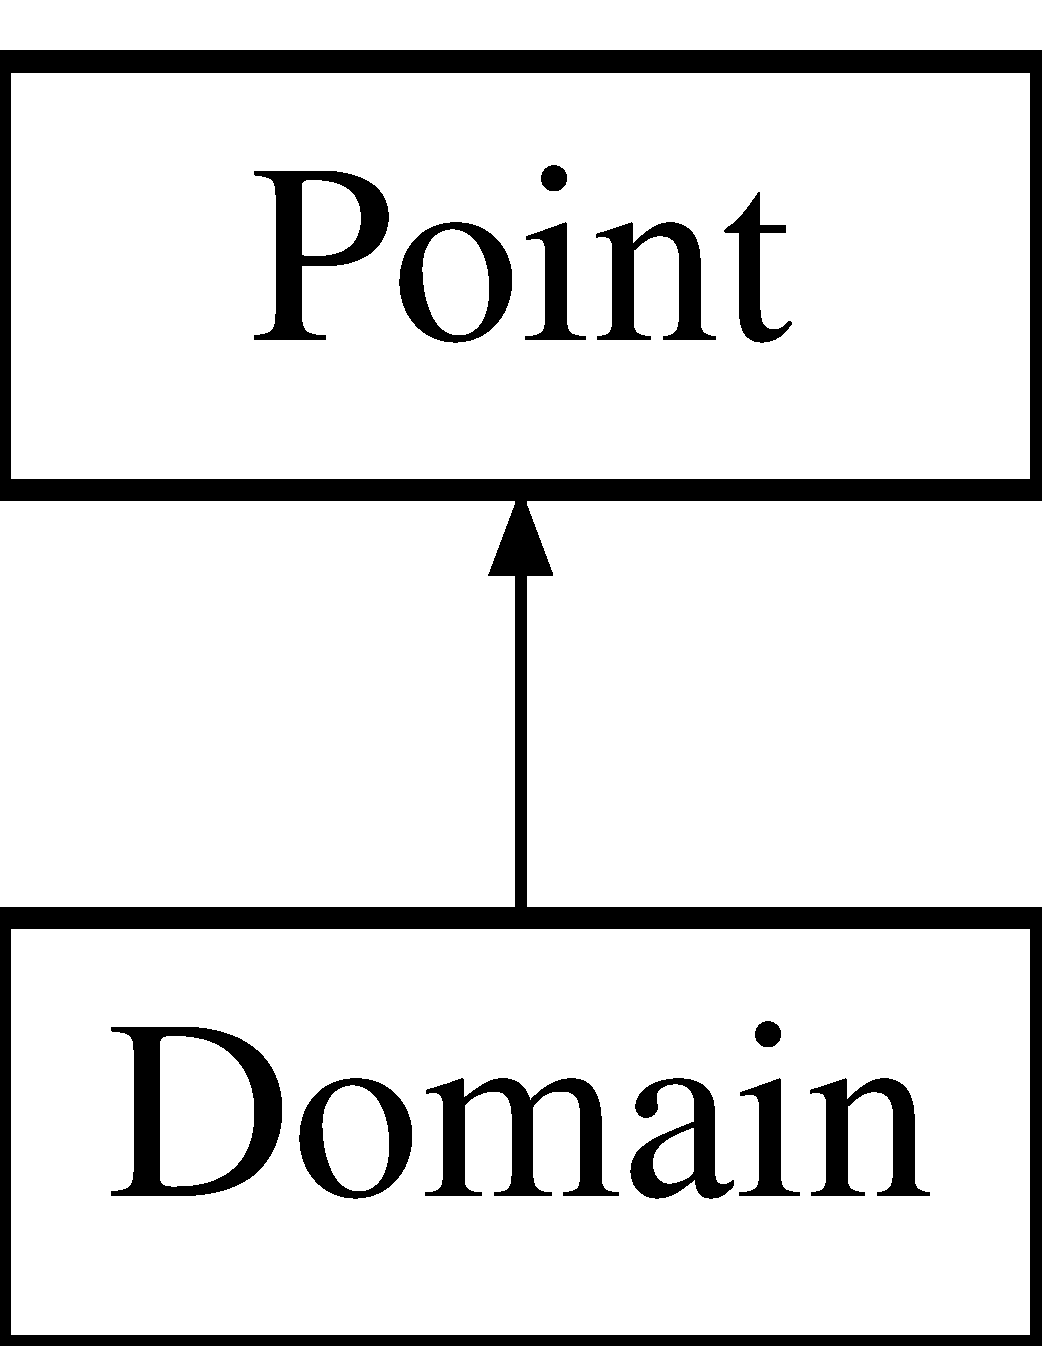
\includegraphics[height=2.000000cm]{class_domain}
\end{center}
\end{figure}
\subsection*{Public Member Functions}
\begin{DoxyCompactItemize}
\item 
int \hyperlink{class_domain_a2aeb4c39576094f7d65be83aae2c48f2}{get\+\_\+compartment\+\_\+number} ()
\item 
void \hyperlink{class_domain_a207d03cc926a3bd612ee76c282ddb10f}{set\+\_\+compartment\+\_\+number} (int i, int j)
\item 
void \hyperlink{class_domain_a4d469609eba2afb4cbaf3810fc34d4e1}{set\+\_\+end} (int i)
\item 
int \hyperlink{class_domain_aeb0bf2fcbaaaa349ce0fb11f192f5cb8}{get\+\_\+end} ()
\item 
void \hyperlink{class_domain_a2c8568b850ff8e59aedb3b66a501b003}{set\+\_\+curve} (int i)
\item 
int \hyperlink{class_domain_aa2278b647f29f47ed2adca466815da59}{get\+\_\+curve} ()
\item 
void \hyperlink{class_domain_a4b33557e861792bb9200707c9eddad1e}{set\+\_\+index} (int i)
\item 
int \hyperlink{class_domain_a24dcaa49a47c41381e46718ed7719e02}{get\+\_\+index} ()
\end{DoxyCompactItemize}
\subsection*{Private Attributes}
\begin{DoxyCompactItemize}
\item 
int \hyperlink{class_domain_ae4a3140523f5101fe60b05dbfc280fe1}{compartment\+\_\+number}
\item 
int \hyperlink{class_domain_af325c2c3f1cfbbae199d10fb8d7486e1}{end}
\item 
int \hyperlink{class_domain_a34957cc9e5ab74e87e7870198eb04ef8}{curve\+\_\+start}
\item 
int \hyperlink{class_domain_a0242b8dac23da9fe639f62bda97ea85c}{index}
\end{DoxyCompactItemize}


\subsection{Member Function Documentation}
\hypertarget{class_domain_a2aeb4c39576094f7d65be83aae2c48f2}{}\index{Domain@{Domain}!get\+\_\+compartment\+\_\+number@{get\+\_\+compartment\+\_\+number}}
\index{get\+\_\+compartment\+\_\+number@{get\+\_\+compartment\+\_\+number}!Domain@{Domain}}
\subsubsection[{get\+\_\+compartment\+\_\+number}]{\setlength{\rightskip}{0pt plus 5cm}int Domain\+::get\+\_\+compartment\+\_\+number (
\begin{DoxyParamCaption}
{}
\end{DoxyParamCaption}
)}\label{class_domain_a2aeb4c39576094f7d65be83aae2c48f2}
\hypertarget{class_domain_aa2278b647f29f47ed2adca466815da59}{}\index{Domain@{Domain}!get\+\_\+curve@{get\+\_\+curve}}
\index{get\+\_\+curve@{get\+\_\+curve}!Domain@{Domain}}
\subsubsection[{get\+\_\+curve}]{\setlength{\rightskip}{0pt plus 5cm}int Domain\+::get\+\_\+curve (
\begin{DoxyParamCaption}
{}
\end{DoxyParamCaption}
)}\label{class_domain_aa2278b647f29f47ed2adca466815da59}
\hypertarget{class_domain_aeb0bf2fcbaaaa349ce0fb11f192f5cb8}{}\index{Domain@{Domain}!get\+\_\+end@{get\+\_\+end}}
\index{get\+\_\+end@{get\+\_\+end}!Domain@{Domain}}
\subsubsection[{get\+\_\+end}]{\setlength{\rightskip}{0pt plus 5cm}int Domain\+::get\+\_\+end (
\begin{DoxyParamCaption}
{}
\end{DoxyParamCaption}
)}\label{class_domain_aeb0bf2fcbaaaa349ce0fb11f192f5cb8}
\hypertarget{class_domain_a24dcaa49a47c41381e46718ed7719e02}{}\index{Domain@{Domain}!get\+\_\+index@{get\+\_\+index}}
\index{get\+\_\+index@{get\+\_\+index}!Domain@{Domain}}
\subsubsection[{get\+\_\+index}]{\setlength{\rightskip}{0pt plus 5cm}int Domain\+::get\+\_\+index (
\begin{DoxyParamCaption}
{}
\end{DoxyParamCaption}
)}\label{class_domain_a24dcaa49a47c41381e46718ed7719e02}
\hypertarget{class_domain_a207d03cc926a3bd612ee76c282ddb10f}{}\index{Domain@{Domain}!set\+\_\+compartment\+\_\+number@{set\+\_\+compartment\+\_\+number}}
\index{set\+\_\+compartment\+\_\+number@{set\+\_\+compartment\+\_\+number}!Domain@{Domain}}
\subsubsection[{set\+\_\+compartment\+\_\+number}]{\setlength{\rightskip}{0pt plus 5cm}void Domain\+::set\+\_\+compartment\+\_\+number (
\begin{DoxyParamCaption}
\item[{int}]{i, }
\item[{int}]{j}
\end{DoxyParamCaption}
)}\label{class_domain_a207d03cc926a3bd612ee76c282ddb10f}
\hypertarget{class_domain_a2c8568b850ff8e59aedb3b66a501b003}{}\index{Domain@{Domain}!set\+\_\+curve@{set\+\_\+curve}}
\index{set\+\_\+curve@{set\+\_\+curve}!Domain@{Domain}}
\subsubsection[{set\+\_\+curve}]{\setlength{\rightskip}{0pt plus 5cm}void Domain\+::set\+\_\+curve (
\begin{DoxyParamCaption}
\item[{int}]{i}
\end{DoxyParamCaption}
)}\label{class_domain_a2c8568b850ff8e59aedb3b66a501b003}
\hypertarget{class_domain_a4d469609eba2afb4cbaf3810fc34d4e1}{}\index{Domain@{Domain}!set\+\_\+end@{set\+\_\+end}}
\index{set\+\_\+end@{set\+\_\+end}!Domain@{Domain}}
\subsubsection[{set\+\_\+end}]{\setlength{\rightskip}{0pt plus 5cm}void Domain\+::set\+\_\+end (
\begin{DoxyParamCaption}
\item[{int}]{i}
\end{DoxyParamCaption}
)}\label{class_domain_a4d469609eba2afb4cbaf3810fc34d4e1}
\hypertarget{class_domain_a4b33557e861792bb9200707c9eddad1e}{}\index{Domain@{Domain}!set\+\_\+index@{set\+\_\+index}}
\index{set\+\_\+index@{set\+\_\+index}!Domain@{Domain}}
\subsubsection[{set\+\_\+index}]{\setlength{\rightskip}{0pt plus 5cm}void Domain\+::set\+\_\+index (
\begin{DoxyParamCaption}
\item[{int}]{i}
\end{DoxyParamCaption}
)}\label{class_domain_a4b33557e861792bb9200707c9eddad1e}


\subsection{Member Data Documentation}
\hypertarget{class_domain_ae4a3140523f5101fe60b05dbfc280fe1}{}\index{Domain@{Domain}!compartment\+\_\+number@{compartment\+\_\+number}}
\index{compartment\+\_\+number@{compartment\+\_\+number}!Domain@{Domain}}
\subsubsection[{compartment\+\_\+number}]{\setlength{\rightskip}{0pt plus 5cm}int Domain\+::compartment\+\_\+number\hspace{0.3cm}{\ttfamily [private]}}\label{class_domain_ae4a3140523f5101fe60b05dbfc280fe1}
\hypertarget{class_domain_a34957cc9e5ab74e87e7870198eb04ef8}{}\index{Domain@{Domain}!curve\+\_\+start@{curve\+\_\+start}}
\index{curve\+\_\+start@{curve\+\_\+start}!Domain@{Domain}}
\subsubsection[{curve\+\_\+start}]{\setlength{\rightskip}{0pt plus 5cm}int Domain\+::curve\+\_\+start\hspace{0.3cm}{\ttfamily [private]}}\label{class_domain_a34957cc9e5ab74e87e7870198eb04ef8}
\hypertarget{class_domain_af325c2c3f1cfbbae199d10fb8d7486e1}{}\index{Domain@{Domain}!end@{end}}
\index{end@{end}!Domain@{Domain}}
\subsubsection[{end}]{\setlength{\rightskip}{0pt plus 5cm}int Domain\+::end\hspace{0.3cm}{\ttfamily [private]}}\label{class_domain_af325c2c3f1cfbbae199d10fb8d7486e1}
\hypertarget{class_domain_a0242b8dac23da9fe639f62bda97ea85c}{}\index{Domain@{Domain}!index@{index}}
\index{index@{index}!Domain@{Domain}}
\subsubsection[{index}]{\setlength{\rightskip}{0pt plus 5cm}int Domain\+::index\hspace{0.3cm}{\ttfamily [private]}}\label{class_domain_a0242b8dac23da9fe639f62bda97ea85c}


The documentation for this class was generated from the following files\+:\begin{DoxyCompactItemize}
\item 
src/\hyperlink{_domain_8h}{Domain.\+h}\item 
src/\hyperlink{_domain_8cpp}{Domain.\+cpp}\end{DoxyCompactItemize}

\hypertarget{class_grid_points}{}\section{Grid\+Points Class Reference}
\label{class_grid_points}\index{Grid\+Points@{Grid\+Points}}


{\ttfamily \#include $<$Grid\+Points.\+h$>$}

\subsection*{Public Member Functions}
\begin{DoxyCompactItemize}
\item 
void \hyperlink{class_grid_points_a557a1de0c4e971a1f00124c12393d35b}{Linear\+\_\+\+Grid} (\hyperlink{class_point}{Point} point1, \hyperlink{class_point}{Point} point2, int N)
\item 
void \hyperlink{class_grid_points_a2cd9f7d761cd106dc340b2a4b10da33c}{Circular\+\_\+\+Grid} (\hyperlink{class_point}{Point} point1, \hyperlink{class_point}{Point} point2, int N)
\item 
void \hyperlink{class_grid_points_ad67d842767dea1f762fffc1d6c4538ca}{Elliptic\+\_\+\+Grid} (\hyperlink{class_point}{Point} point1, \hyperlink{class_point}{Point} point2, int N)
\item 
void \hyperlink{class_grid_points_a7f8ba8461891af5a041deea1c6aa485c}{Parabolic\+\_\+\+Grid} (\hyperlink{class_point}{Point} point1, \hyperlink{class_point}{Point} point2, int N)
\item 
void \hyperlink{class_grid_points_a33d1514a1b36ae513bda9332bf8207ab}{Exponential\+\_\+\+Grid} (\hyperlink{class_point}{Point} point1, \hyperlink{class_point}{Point} point2, int N)
\item 
void \hyperlink{class_grid_points_a5961d7f154d16819467211a92f51a480}{Quadratic\+\_\+\+Grid} (\hyperlink{class_point}{Point} point1, \hyperlink{class_point}{Point} point2, int N)
\end{DoxyCompactItemize}
\subsection*{Public Attributes}
\begin{DoxyCompactItemize}
\item 
\hyperlink{class_point}{Point} $\ast$ \hyperlink{class_grid_points_aeb3801fe3a61a3c14fa9e23ad93b815d}{grid\+\_\+points}
\end{DoxyCompactItemize}
\subsection*{Private Member Functions}
\begin{DoxyCompactItemize}
\item 
float \hyperlink{class_grid_points_a85035aa63c904cc066802c13c18d465e}{get\+Angle} (\hyperlink{class_point}{Point} point1, \hyperlink{class_point}{Point} point2)
\item 
float \hyperlink{class_grid_points_a9b32f73ce9f10c09c97069816c1253f0}{get\+Radius} (\hyperlink{class_point}{Point} point1, \hyperlink{class_point}{Point} center)
\item 
void \hyperlink{class_grid_points_a007b5f15c63c07f6c0101db9e42e26fa}{divide\+\_\+domain\+\_\+\+Line} (\hyperlink{class_point}{Point} point1, \hyperlink{class_point}{Point} point2, int N)
\item 
void \hyperlink{class_grid_points_a8910c072b4a9839f912513a4bbf517c0}{divide\+\_\+domain\+\_\+\+Circle} (\hyperlink{class_point}{Point} point1, \hyperlink{class_point}{Point} point2, int N, bool direction)
\item 
void \hyperlink{class_grid_points_a353c592f1a0bffc5bee6e240afb7ce63}{divide\+\_\+domain\+\_\+\+Ellipse} (\hyperlink{class_point}{Point} point1, \hyperlink{class_point}{Point} point2, int N, bool direction)
\item 
void \hyperlink{class_grid_points_aad9b87e262e10af26a9925ccc9f0cc30}{divide\+\_\+domain\+\_\+\+Parabola} (\hyperlink{class_point}{Point} point1, \hyperlink{class_point}{Point} point2, int N)
\item 
void \hyperlink{class_grid_points_a3d273573aa628b70644a694a50d9b696}{divide\+\_\+domain\+\_\+exponential} (\hyperlink{class_point}{Point} point1, \hyperlink{class_point}{Point} point2, int N)
\item 
void \hyperlink{class_grid_points_a16e4eb481007bf863d78b930b836eb23}{divide\+\_\+domain\+\_\+\+Quadratic} (\hyperlink{class_point}{Point} point1, \hyperlink{class_point}{Point} point2, int N)
\item 
bool \hyperlink{class_grid_points_a5babb6d204dcab7adcc25715eba8b0e6}{get\+\_\+direction} ()
\end{DoxyCompactItemize}


\subsection{Member Function Documentation}
\hypertarget{class_grid_points_a2cd9f7d761cd106dc340b2a4b10da33c}{}\index{Grid\+Points@{Grid\+Points}!Circular\+\_\+\+Grid@{Circular\+\_\+\+Grid}}
\index{Circular\+\_\+\+Grid@{Circular\+\_\+\+Grid}!Grid\+Points@{Grid\+Points}}
\subsubsection[{Circular\+\_\+\+Grid}]{\setlength{\rightskip}{0pt plus 5cm}void Grid\+Points\+::\+Circular\+\_\+\+Grid (
\begin{DoxyParamCaption}
\item[{{\bf Point}}]{point1, }
\item[{{\bf Point}}]{point2, }
\item[{int}]{N}
\end{DoxyParamCaption}
)}\label{class_grid_points_a2cd9f7d761cd106dc340b2a4b10da33c}
\hypertarget{class_grid_points_a8910c072b4a9839f912513a4bbf517c0}{}\index{Grid\+Points@{Grid\+Points}!divide\+\_\+domain\+\_\+\+Circle@{divide\+\_\+domain\+\_\+\+Circle}}
\index{divide\+\_\+domain\+\_\+\+Circle@{divide\+\_\+domain\+\_\+\+Circle}!Grid\+Points@{Grid\+Points}}
\subsubsection[{divide\+\_\+domain\+\_\+\+Circle}]{\setlength{\rightskip}{0pt plus 5cm}void Grid\+Points\+::divide\+\_\+domain\+\_\+\+Circle (
\begin{DoxyParamCaption}
\item[{{\bf Point}}]{point1, }
\item[{{\bf Point}}]{point2, }
\item[{int}]{N, }
\item[{bool}]{direction}
\end{DoxyParamCaption}
)\hspace{0.3cm}{\ttfamily [private]}}\label{class_grid_points_a8910c072b4a9839f912513a4bbf517c0}
\hypertarget{class_grid_points_a353c592f1a0bffc5bee6e240afb7ce63}{}\index{Grid\+Points@{Grid\+Points}!divide\+\_\+domain\+\_\+\+Ellipse@{divide\+\_\+domain\+\_\+\+Ellipse}}
\index{divide\+\_\+domain\+\_\+\+Ellipse@{divide\+\_\+domain\+\_\+\+Ellipse}!Grid\+Points@{Grid\+Points}}
\subsubsection[{divide\+\_\+domain\+\_\+\+Ellipse}]{\setlength{\rightskip}{0pt plus 5cm}void Grid\+Points\+::divide\+\_\+domain\+\_\+\+Ellipse (
\begin{DoxyParamCaption}
\item[{{\bf Point}}]{point1, }
\item[{{\bf Point}}]{point2, }
\item[{int}]{N, }
\item[{bool}]{direction}
\end{DoxyParamCaption}
)\hspace{0.3cm}{\ttfamily [private]}}\label{class_grid_points_a353c592f1a0bffc5bee6e240afb7ce63}
\hypertarget{class_grid_points_a3d273573aa628b70644a694a50d9b696}{}\index{Grid\+Points@{Grid\+Points}!divide\+\_\+domain\+\_\+exponential@{divide\+\_\+domain\+\_\+exponential}}
\index{divide\+\_\+domain\+\_\+exponential@{divide\+\_\+domain\+\_\+exponential}!Grid\+Points@{Grid\+Points}}
\subsubsection[{divide\+\_\+domain\+\_\+exponential}]{\setlength{\rightskip}{0pt plus 5cm}void Grid\+Points\+::divide\+\_\+domain\+\_\+exponential (
\begin{DoxyParamCaption}
\item[{{\bf Point}}]{point1, }
\item[{{\bf Point}}]{point2, }
\item[{int}]{N}
\end{DoxyParamCaption}
)\hspace{0.3cm}{\ttfamily [private]}}\label{class_grid_points_a3d273573aa628b70644a694a50d9b696}
\hypertarget{class_grid_points_a007b5f15c63c07f6c0101db9e42e26fa}{}\index{Grid\+Points@{Grid\+Points}!divide\+\_\+domain\+\_\+\+Line@{divide\+\_\+domain\+\_\+\+Line}}
\index{divide\+\_\+domain\+\_\+\+Line@{divide\+\_\+domain\+\_\+\+Line}!Grid\+Points@{Grid\+Points}}
\subsubsection[{divide\+\_\+domain\+\_\+\+Line}]{\setlength{\rightskip}{0pt plus 5cm}void Grid\+Points\+::divide\+\_\+domain\+\_\+\+Line (
\begin{DoxyParamCaption}
\item[{{\bf Point}}]{point1, }
\item[{{\bf Point}}]{point2, }
\item[{int}]{N}
\end{DoxyParamCaption}
)\hspace{0.3cm}{\ttfamily [private]}}\label{class_grid_points_a007b5f15c63c07f6c0101db9e42e26fa}
\hypertarget{class_grid_points_aad9b87e262e10af26a9925ccc9f0cc30}{}\index{Grid\+Points@{Grid\+Points}!divide\+\_\+domain\+\_\+\+Parabola@{divide\+\_\+domain\+\_\+\+Parabola}}
\index{divide\+\_\+domain\+\_\+\+Parabola@{divide\+\_\+domain\+\_\+\+Parabola}!Grid\+Points@{Grid\+Points}}
\subsubsection[{divide\+\_\+domain\+\_\+\+Parabola}]{\setlength{\rightskip}{0pt plus 5cm}void Grid\+Points\+::divide\+\_\+domain\+\_\+\+Parabola (
\begin{DoxyParamCaption}
\item[{{\bf Point}}]{point1, }
\item[{{\bf Point}}]{point2, }
\item[{int}]{N}
\end{DoxyParamCaption}
)\hspace{0.3cm}{\ttfamily [private]}}\label{class_grid_points_aad9b87e262e10af26a9925ccc9f0cc30}
\hypertarget{class_grid_points_a16e4eb481007bf863d78b930b836eb23}{}\index{Grid\+Points@{Grid\+Points}!divide\+\_\+domain\+\_\+\+Quadratic@{divide\+\_\+domain\+\_\+\+Quadratic}}
\index{divide\+\_\+domain\+\_\+\+Quadratic@{divide\+\_\+domain\+\_\+\+Quadratic}!Grid\+Points@{Grid\+Points}}
\subsubsection[{divide\+\_\+domain\+\_\+\+Quadratic}]{\setlength{\rightskip}{0pt plus 5cm}void Grid\+Points\+::divide\+\_\+domain\+\_\+\+Quadratic (
\begin{DoxyParamCaption}
\item[{{\bf Point}}]{point1, }
\item[{{\bf Point}}]{point2, }
\item[{int}]{N}
\end{DoxyParamCaption}
)\hspace{0.3cm}{\ttfamily [private]}}\label{class_grid_points_a16e4eb481007bf863d78b930b836eb23}
\hypertarget{class_grid_points_ad67d842767dea1f762fffc1d6c4538ca}{}\index{Grid\+Points@{Grid\+Points}!Elliptic\+\_\+\+Grid@{Elliptic\+\_\+\+Grid}}
\index{Elliptic\+\_\+\+Grid@{Elliptic\+\_\+\+Grid}!Grid\+Points@{Grid\+Points}}
\subsubsection[{Elliptic\+\_\+\+Grid}]{\setlength{\rightskip}{0pt plus 5cm}void Grid\+Points\+::\+Elliptic\+\_\+\+Grid (
\begin{DoxyParamCaption}
\item[{{\bf Point}}]{point1, }
\item[{{\bf Point}}]{point2, }
\item[{int}]{N}
\end{DoxyParamCaption}
)}\label{class_grid_points_ad67d842767dea1f762fffc1d6c4538ca}
\hypertarget{class_grid_points_a33d1514a1b36ae513bda9332bf8207ab}{}\index{Grid\+Points@{Grid\+Points}!Exponential\+\_\+\+Grid@{Exponential\+\_\+\+Grid}}
\index{Exponential\+\_\+\+Grid@{Exponential\+\_\+\+Grid}!Grid\+Points@{Grid\+Points}}
\subsubsection[{Exponential\+\_\+\+Grid}]{\setlength{\rightskip}{0pt plus 5cm}void Grid\+Points\+::\+Exponential\+\_\+\+Grid (
\begin{DoxyParamCaption}
\item[{{\bf Point}}]{point1, }
\item[{{\bf Point}}]{point2, }
\item[{int}]{N}
\end{DoxyParamCaption}
)}\label{class_grid_points_a33d1514a1b36ae513bda9332bf8207ab}
\hypertarget{class_grid_points_a5babb6d204dcab7adcc25715eba8b0e6}{}\index{Grid\+Points@{Grid\+Points}!get\+\_\+direction@{get\+\_\+direction}}
\index{get\+\_\+direction@{get\+\_\+direction}!Grid\+Points@{Grid\+Points}}
\subsubsection[{get\+\_\+direction}]{\setlength{\rightskip}{0pt plus 5cm}bool Grid\+Points\+::get\+\_\+direction (
\begin{DoxyParamCaption}
{}
\end{DoxyParamCaption}
)\hspace{0.3cm}{\ttfamily [private]}}\label{class_grid_points_a5babb6d204dcab7adcc25715eba8b0e6}
\hypertarget{class_grid_points_a85035aa63c904cc066802c13c18d465e}{}\index{Grid\+Points@{Grid\+Points}!get\+Angle@{get\+Angle}}
\index{get\+Angle@{get\+Angle}!Grid\+Points@{Grid\+Points}}
\subsubsection[{get\+Angle}]{\setlength{\rightskip}{0pt plus 5cm}float Grid\+Points\+::get\+Angle (
\begin{DoxyParamCaption}
\item[{{\bf Point}}]{point1, }
\item[{{\bf Point}}]{point2}
\end{DoxyParamCaption}
)\hspace{0.3cm}{\ttfamily [private]}}\label{class_grid_points_a85035aa63c904cc066802c13c18d465e}
\hypertarget{class_grid_points_a9b32f73ce9f10c09c97069816c1253f0}{}\index{Grid\+Points@{Grid\+Points}!get\+Radius@{get\+Radius}}
\index{get\+Radius@{get\+Radius}!Grid\+Points@{Grid\+Points}}
\subsubsection[{get\+Radius}]{\setlength{\rightskip}{0pt plus 5cm}float Grid\+Points\+::get\+Radius (
\begin{DoxyParamCaption}
\item[{{\bf Point}}]{point1, }
\item[{{\bf Point}}]{center}
\end{DoxyParamCaption}
)\hspace{0.3cm}{\ttfamily [private]}}\label{class_grid_points_a9b32f73ce9f10c09c97069816c1253f0}
\hypertarget{class_grid_points_a557a1de0c4e971a1f00124c12393d35b}{}\index{Grid\+Points@{Grid\+Points}!Linear\+\_\+\+Grid@{Linear\+\_\+\+Grid}}
\index{Linear\+\_\+\+Grid@{Linear\+\_\+\+Grid}!Grid\+Points@{Grid\+Points}}
\subsubsection[{Linear\+\_\+\+Grid}]{\setlength{\rightskip}{0pt plus 5cm}void Grid\+Points\+::\+Linear\+\_\+\+Grid (
\begin{DoxyParamCaption}
\item[{{\bf Point}}]{point1, }
\item[{{\bf Point}}]{point2, }
\item[{int}]{N}
\end{DoxyParamCaption}
)}\label{class_grid_points_a557a1de0c4e971a1f00124c12393d35b}
\hypertarget{class_grid_points_a7f8ba8461891af5a041deea1c6aa485c}{}\index{Grid\+Points@{Grid\+Points}!Parabolic\+\_\+\+Grid@{Parabolic\+\_\+\+Grid}}
\index{Parabolic\+\_\+\+Grid@{Parabolic\+\_\+\+Grid}!Grid\+Points@{Grid\+Points}}
\subsubsection[{Parabolic\+\_\+\+Grid}]{\setlength{\rightskip}{0pt plus 5cm}void Grid\+Points\+::\+Parabolic\+\_\+\+Grid (
\begin{DoxyParamCaption}
\item[{{\bf Point}}]{point1, }
\item[{{\bf Point}}]{point2, }
\item[{int}]{N}
\end{DoxyParamCaption}
)}\label{class_grid_points_a7f8ba8461891af5a041deea1c6aa485c}
\hypertarget{class_grid_points_a5961d7f154d16819467211a92f51a480}{}\index{Grid\+Points@{Grid\+Points}!Quadratic\+\_\+\+Grid@{Quadratic\+\_\+\+Grid}}
\index{Quadratic\+\_\+\+Grid@{Quadratic\+\_\+\+Grid}!Grid\+Points@{Grid\+Points}}
\subsubsection[{Quadratic\+\_\+\+Grid}]{\setlength{\rightskip}{0pt plus 5cm}void Grid\+Points\+::\+Quadratic\+\_\+\+Grid (
\begin{DoxyParamCaption}
\item[{{\bf Point}}]{point1, }
\item[{{\bf Point}}]{point2, }
\item[{int}]{N}
\end{DoxyParamCaption}
)}\label{class_grid_points_a5961d7f154d16819467211a92f51a480}


\subsection{Member Data Documentation}
\hypertarget{class_grid_points_aeb3801fe3a61a3c14fa9e23ad93b815d}{}\index{Grid\+Points@{Grid\+Points}!grid\+\_\+points@{grid\+\_\+points}}
\index{grid\+\_\+points@{grid\+\_\+points}!Grid\+Points@{Grid\+Points}}
\subsubsection[{grid\+\_\+points}]{\setlength{\rightskip}{0pt plus 5cm}{\bf Point}$\ast$ Grid\+Points\+::grid\+\_\+points}\label{class_grid_points_aeb3801fe3a61a3c14fa9e23ad93b815d}


The documentation for this class was generated from the following files\+:\begin{DoxyCompactItemize}
\item 
src/\hyperlink{_grid_points_8h}{Grid\+Points.\+h}\item 
src/\hyperlink{_grid_points_8cpp}{Grid\+Points.\+cpp}\end{DoxyCompactItemize}

\hypertarget{class_point}{}\section{Point Class Reference}
\label{class_point}\index{Point@{Point}}


{\ttfamily \#include $<$Point.\+h$>$}

Inheritance diagram for Point\+:\begin{figure}[H]
\begin{center}
\leavevmode
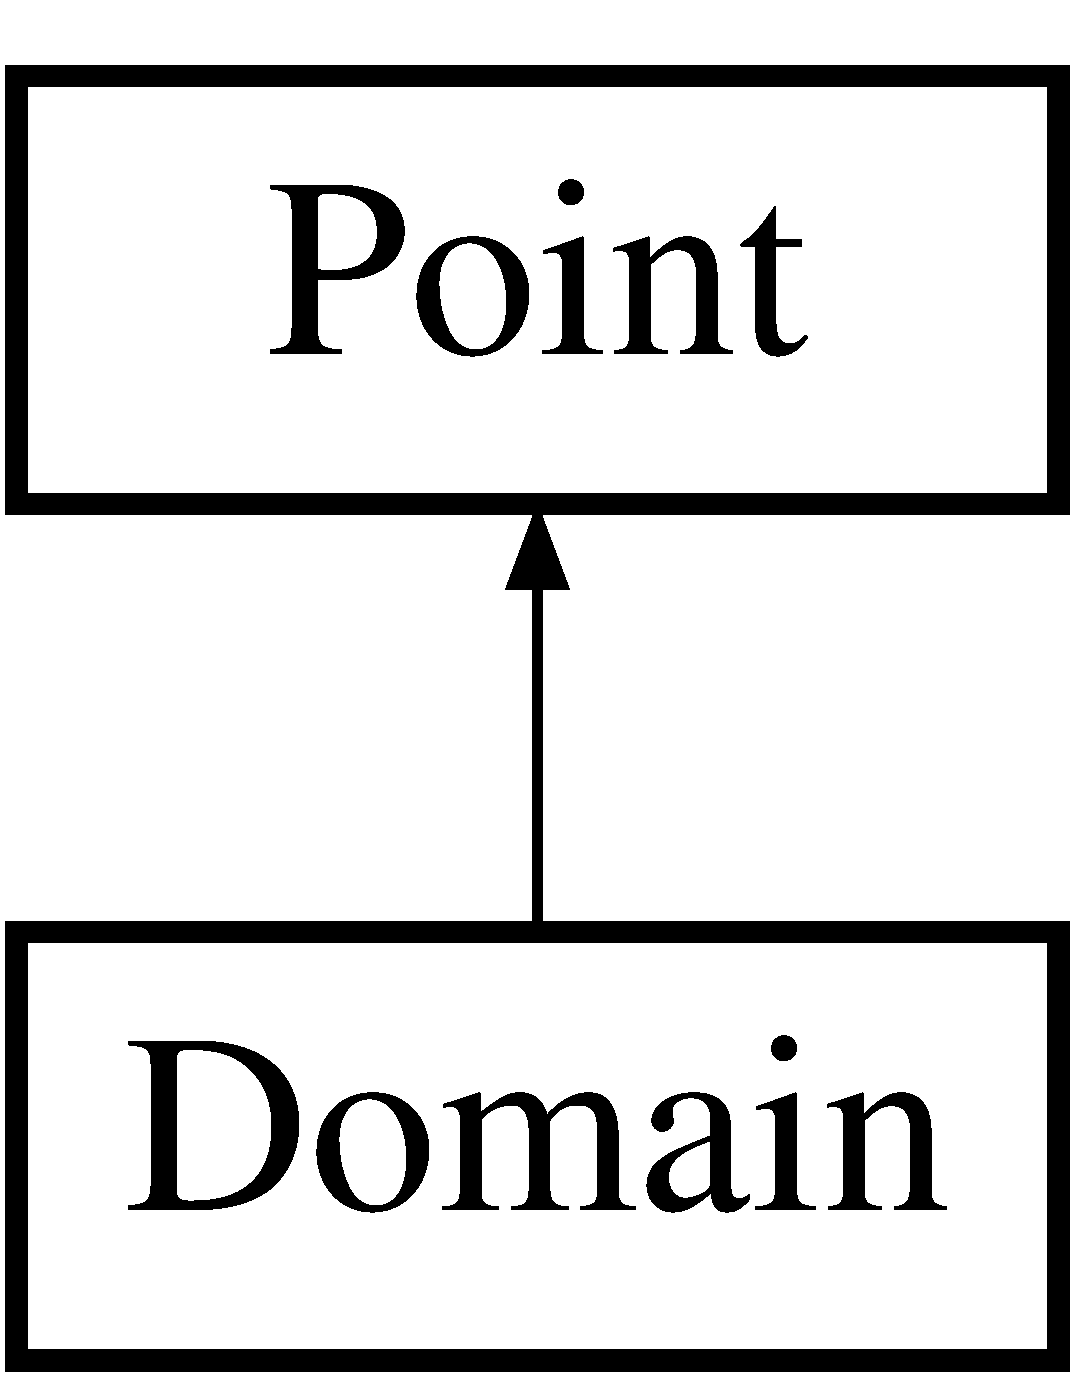
\includegraphics[height=2.000000cm]{class_point}
\end{center}
\end{figure}
\subsection*{Public Member Functions}
\begin{DoxyCompactItemize}
\item 
void \hyperlink{class_point_adcd81f44e0e8c78a25e6f6b86ca6c1ad}{get\+\_\+\+Coordinate} (float x, float y)
\item 
float \hyperlink{class_point_a7d159f63afcd03d45664bd91536f20d7}{get\+\_\+x\+\_\+coordinate} ()
\item 
float \hyperlink{class_point_a2339ebeb267c722dda118fd17d7d44a6}{get\+\_\+y\+\_\+coordinate} ()
\item 
void \hyperlink{class_point_a24af58a3a60559c2dfbadda4874db051}{get\+\_\+\+Point} ()
\item 
void \hyperlink{class_point_ad3999e6f2ca20182a4a45a4b1fa7be87}{display} ()
\end{DoxyCompactItemize}
\subsection*{Private Attributes}
\begin{DoxyCompactItemize}
\item 
float \hyperlink{class_point_a49bfb2a75e9352d61a0b5cb03ed594ee}{coordinate\+\_\+x}
\item 
float \hyperlink{class_point_a4aa8b15f92a9a3c73fa64e74c1086906}{coordinate\+\_\+y}
\end{DoxyCompactItemize}


\subsection{Member Function Documentation}
\hypertarget{class_point_ad3999e6f2ca20182a4a45a4b1fa7be87}{}\index{Point@{Point}!display@{display}}
\index{display@{display}!Point@{Point}}
\subsubsection[{display}]{\setlength{\rightskip}{0pt plus 5cm}void Point\+::display (
\begin{DoxyParamCaption}
{}
\end{DoxyParamCaption}
)}\label{class_point_ad3999e6f2ca20182a4a45a4b1fa7be87}
\hypertarget{class_point_adcd81f44e0e8c78a25e6f6b86ca6c1ad}{}\index{Point@{Point}!get\+\_\+\+Coordinate@{get\+\_\+\+Coordinate}}
\index{get\+\_\+\+Coordinate@{get\+\_\+\+Coordinate}!Point@{Point}}
\subsubsection[{get\+\_\+\+Coordinate}]{\setlength{\rightskip}{0pt plus 5cm}void Point\+::get\+\_\+\+Coordinate (
\begin{DoxyParamCaption}
\item[{float}]{x, }
\item[{float}]{y}
\end{DoxyParamCaption}
)}\label{class_point_adcd81f44e0e8c78a25e6f6b86ca6c1ad}
\hypertarget{class_point_a24af58a3a60559c2dfbadda4874db051}{}\index{Point@{Point}!get\+\_\+\+Point@{get\+\_\+\+Point}}
\index{get\+\_\+\+Point@{get\+\_\+\+Point}!Point@{Point}}
\subsubsection[{get\+\_\+\+Point}]{\setlength{\rightskip}{0pt plus 5cm}void Point\+::get\+\_\+\+Point (
\begin{DoxyParamCaption}
{}
\end{DoxyParamCaption}
)}\label{class_point_a24af58a3a60559c2dfbadda4874db051}
\hypertarget{class_point_a7d159f63afcd03d45664bd91536f20d7}{}\index{Point@{Point}!get\+\_\+x\+\_\+coordinate@{get\+\_\+x\+\_\+coordinate}}
\index{get\+\_\+x\+\_\+coordinate@{get\+\_\+x\+\_\+coordinate}!Point@{Point}}
\subsubsection[{get\+\_\+x\+\_\+coordinate}]{\setlength{\rightskip}{0pt plus 5cm}float Point\+::get\+\_\+x\+\_\+coordinate (
\begin{DoxyParamCaption}
{}
\end{DoxyParamCaption}
)}\label{class_point_a7d159f63afcd03d45664bd91536f20d7}
\hypertarget{class_point_a2339ebeb267c722dda118fd17d7d44a6}{}\index{Point@{Point}!get\+\_\+y\+\_\+coordinate@{get\+\_\+y\+\_\+coordinate}}
\index{get\+\_\+y\+\_\+coordinate@{get\+\_\+y\+\_\+coordinate}!Point@{Point}}
\subsubsection[{get\+\_\+y\+\_\+coordinate}]{\setlength{\rightskip}{0pt plus 5cm}float Point\+::get\+\_\+y\+\_\+coordinate (
\begin{DoxyParamCaption}
{}
\end{DoxyParamCaption}
)}\label{class_point_a2339ebeb267c722dda118fd17d7d44a6}


\subsection{Member Data Documentation}
\hypertarget{class_point_a49bfb2a75e9352d61a0b5cb03ed594ee}{}\index{Point@{Point}!coordinate\+\_\+x@{coordinate\+\_\+x}}
\index{coordinate\+\_\+x@{coordinate\+\_\+x}!Point@{Point}}
\subsubsection[{coordinate\+\_\+x}]{\setlength{\rightskip}{0pt plus 5cm}float Point\+::coordinate\+\_\+x\hspace{0.3cm}{\ttfamily [private]}}\label{class_point_a49bfb2a75e9352d61a0b5cb03ed594ee}
\hypertarget{class_point_a4aa8b15f92a9a3c73fa64e74c1086906}{}\index{Point@{Point}!coordinate\+\_\+y@{coordinate\+\_\+y}}
\index{coordinate\+\_\+y@{coordinate\+\_\+y}!Point@{Point}}
\subsubsection[{coordinate\+\_\+y}]{\setlength{\rightskip}{0pt plus 5cm}float Point\+::coordinate\+\_\+y\hspace{0.3cm}{\ttfamily [private]}}\label{class_point_a4aa8b15f92a9a3c73fa64e74c1086906}


The documentation for this class was generated from the following files\+:\begin{DoxyCompactItemize}
\item 
src/\hyperlink{_point_8h}{Point.\+h}\item 
src/\hyperlink{_point_8cpp}{Point.\+cpp}\end{DoxyCompactItemize}

\hypertarget{class_sparse___matrix}{}\section{Sparse\+\_\+\+Matrix Class Reference}
\label{class_sparse___matrix}\index{Sparse\+\_\+\+Matrix@{Sparse\+\_\+\+Matrix}}


{\ttfamily \#include $<$Sparse\+Matrix.\+h$>$}

\subsection*{Public Member Functions}
\begin{DoxyCompactItemize}
\item 
\hyperlink{class_sparse___matrix_aa3ce6db5b1c26f93f86ffb8884dc85bb}{Sparse\+\_\+\+Matrix} (int N)
\item 
void \hyperlink{class_sparse___matrix_a74953876a03a361211af1f8662a8fbc7}{get\+Data} ()
\item 
void \hyperlink{class_sparse___matrix_a686021f48aea779d990ebb647074464c}{initialize} ()
\item 
void \hyperlink{class_sparse___matrix_af1141a3e469a1ab0e95ea58dfee1f96a}{resize} ()
\end{DoxyCompactItemize}
\subsection*{Private Attributes}
\begin{DoxyCompactItemize}
\item 
int \hyperlink{class_sparse___matrix_a0593a57ade44950748c5c9cb5d9d19d6}{size}
\item 
int \hyperlink{class_sparse___matrix_a279885c2e74db32d7f0e89809041b78e}{number\+\_\+non\+\_\+zero}
\item 
int \hyperlink{class_sparse___matrix_abff04b96a095b67b06635ef50c171456}{counter}
\item 
float $\ast$ \hyperlink{class_sparse___matrix_a46b0a2ca128b883175d8e1f03c03c6cc}{A}
\item 
int $\ast$ \hyperlink{class_sparse___matrix_a00f4239303268686d1370ed2d0e52c8d}{I}
\item 
int $\ast$ \hyperlink{class_sparse___matrix_ab7776df86910c160916338d34b53d461}{J}
\end{DoxyCompactItemize}


\subsection{Constructor \& Destructor Documentation}
\hypertarget{class_sparse___matrix_aa3ce6db5b1c26f93f86ffb8884dc85bb}{}\index{Sparse\+\_\+\+Matrix@{Sparse\+\_\+\+Matrix}!Sparse\+\_\+\+Matrix@{Sparse\+\_\+\+Matrix}}
\index{Sparse\+\_\+\+Matrix@{Sparse\+\_\+\+Matrix}!Sparse\+\_\+\+Matrix@{Sparse\+\_\+\+Matrix}}
\subsubsection[{Sparse\+\_\+\+Matrix}]{\setlength{\rightskip}{0pt plus 5cm}Sparse\+\_\+\+Matrix\+::\+Sparse\+\_\+\+Matrix (
\begin{DoxyParamCaption}
\item[{int}]{N}
\end{DoxyParamCaption}
)}\label{class_sparse___matrix_aa3ce6db5b1c26f93f86ffb8884dc85bb}


\subsection{Member Function Documentation}
\hypertarget{class_sparse___matrix_a74953876a03a361211af1f8662a8fbc7}{}\index{Sparse\+\_\+\+Matrix@{Sparse\+\_\+\+Matrix}!get\+Data@{get\+Data}}
\index{get\+Data@{get\+Data}!Sparse\+\_\+\+Matrix@{Sparse\+\_\+\+Matrix}}
\subsubsection[{get\+Data}]{\setlength{\rightskip}{0pt plus 5cm}void Sparse\+\_\+\+Matrix\+::get\+Data (
\begin{DoxyParamCaption}
{}
\end{DoxyParamCaption}
)}\label{class_sparse___matrix_a74953876a03a361211af1f8662a8fbc7}
\hypertarget{class_sparse___matrix_a686021f48aea779d990ebb647074464c}{}\index{Sparse\+\_\+\+Matrix@{Sparse\+\_\+\+Matrix}!initialize@{initialize}}
\index{initialize@{initialize}!Sparse\+\_\+\+Matrix@{Sparse\+\_\+\+Matrix}}
\subsubsection[{initialize}]{\setlength{\rightskip}{0pt plus 5cm}void Sparse\+\_\+\+Matrix\+::initialize (
\begin{DoxyParamCaption}
{}
\end{DoxyParamCaption}
)}\label{class_sparse___matrix_a686021f48aea779d990ebb647074464c}
\hypertarget{class_sparse___matrix_af1141a3e469a1ab0e95ea58dfee1f96a}{}\index{Sparse\+\_\+\+Matrix@{Sparse\+\_\+\+Matrix}!resize@{resize}}
\index{resize@{resize}!Sparse\+\_\+\+Matrix@{Sparse\+\_\+\+Matrix}}
\subsubsection[{resize}]{\setlength{\rightskip}{0pt plus 5cm}void Sparse\+\_\+\+Matrix\+::resize (
\begin{DoxyParamCaption}
{}
\end{DoxyParamCaption}
)}\label{class_sparse___matrix_af1141a3e469a1ab0e95ea58dfee1f96a}


\subsection{Member Data Documentation}
\hypertarget{class_sparse___matrix_a46b0a2ca128b883175d8e1f03c03c6cc}{}\index{Sparse\+\_\+\+Matrix@{Sparse\+\_\+\+Matrix}!A@{A}}
\index{A@{A}!Sparse\+\_\+\+Matrix@{Sparse\+\_\+\+Matrix}}
\subsubsection[{A}]{\setlength{\rightskip}{0pt plus 5cm}float$\ast$ Sparse\+\_\+\+Matrix\+::\+A\hspace{0.3cm}{\ttfamily [private]}}\label{class_sparse___matrix_a46b0a2ca128b883175d8e1f03c03c6cc}
\hypertarget{class_sparse___matrix_abff04b96a095b67b06635ef50c171456}{}\index{Sparse\+\_\+\+Matrix@{Sparse\+\_\+\+Matrix}!counter@{counter}}
\index{counter@{counter}!Sparse\+\_\+\+Matrix@{Sparse\+\_\+\+Matrix}}
\subsubsection[{counter}]{\setlength{\rightskip}{0pt plus 5cm}int Sparse\+\_\+\+Matrix\+::counter\hspace{0.3cm}{\ttfamily [private]}}\label{class_sparse___matrix_abff04b96a095b67b06635ef50c171456}
\hypertarget{class_sparse___matrix_a00f4239303268686d1370ed2d0e52c8d}{}\index{Sparse\+\_\+\+Matrix@{Sparse\+\_\+\+Matrix}!I@{I}}
\index{I@{I}!Sparse\+\_\+\+Matrix@{Sparse\+\_\+\+Matrix}}
\subsubsection[{I}]{\setlength{\rightskip}{0pt plus 5cm}int$\ast$ Sparse\+\_\+\+Matrix\+::\+I\hspace{0.3cm}{\ttfamily [private]}}\label{class_sparse___matrix_a00f4239303268686d1370ed2d0e52c8d}
\hypertarget{class_sparse___matrix_ab7776df86910c160916338d34b53d461}{}\index{Sparse\+\_\+\+Matrix@{Sparse\+\_\+\+Matrix}!J@{J}}
\index{J@{J}!Sparse\+\_\+\+Matrix@{Sparse\+\_\+\+Matrix}}
\subsubsection[{J}]{\setlength{\rightskip}{0pt plus 5cm}int$\ast$ Sparse\+\_\+\+Matrix\+::\+J\hspace{0.3cm}{\ttfamily [private]}}\label{class_sparse___matrix_ab7776df86910c160916338d34b53d461}
\hypertarget{class_sparse___matrix_a279885c2e74db32d7f0e89809041b78e}{}\index{Sparse\+\_\+\+Matrix@{Sparse\+\_\+\+Matrix}!number\+\_\+non\+\_\+zero@{number\+\_\+non\+\_\+zero}}
\index{number\+\_\+non\+\_\+zero@{number\+\_\+non\+\_\+zero}!Sparse\+\_\+\+Matrix@{Sparse\+\_\+\+Matrix}}
\subsubsection[{number\+\_\+non\+\_\+zero}]{\setlength{\rightskip}{0pt plus 5cm}int Sparse\+\_\+\+Matrix\+::number\+\_\+non\+\_\+zero\hspace{0.3cm}{\ttfamily [private]}}\label{class_sparse___matrix_a279885c2e74db32d7f0e89809041b78e}
\hypertarget{class_sparse___matrix_a0593a57ade44950748c5c9cb5d9d19d6}{}\index{Sparse\+\_\+\+Matrix@{Sparse\+\_\+\+Matrix}!size@{size}}
\index{size@{size}!Sparse\+\_\+\+Matrix@{Sparse\+\_\+\+Matrix}}
\subsubsection[{size}]{\setlength{\rightskip}{0pt plus 5cm}int Sparse\+\_\+\+Matrix\+::size\hspace{0.3cm}{\ttfamily [private]}}\label{class_sparse___matrix_a0593a57ade44950748c5c9cb5d9d19d6}


The documentation for this class was generated from the following file\+:\begin{DoxyCompactItemize}
\item 
src/\hyperlink{_sparse_matrix_8h}{Sparse\+Matrix.\+h}\end{DoxyCompactItemize}

\hypertarget{class_vector}{}\section{Vector$<$ T $>$ Class Template Reference}
\label{class_vector}\index{Vector$<$ T $>$@{Vector$<$ T $>$}}


{\ttfamily \#include $<$Vector.\+h$>$}

\subsection*{Public Member Functions}
\begin{DoxyCompactItemize}
\item 
\hyperlink{class_vector_a39d6069675db4ecfc1ab81d440da759a}{Vector} ()
\begin{DoxyCompactList}\small\item\em Default Constructor. \end{DoxyCompactList}\item 
\hyperlink{class_vector_a7233eaf600bca59dbd1a195ccb465cf5}{Vector} (int m)
\begin{DoxyCompactList}\small\item\em Constructor. \end{DoxyCompactList}\item 
\hyperlink{class_vector_aadd88501ee4d48b6da9fa12530373b63}{$\sim$\+Vector} ()
\begin{DoxyCompactList}\small\item\em Destructor. \end{DoxyCompactList}\item 
void \hyperlink{class_vector_af8fbb7be7e884bbd38fd619f791a493b}{display} ()
\begin{DoxyCompactList}\small\item\em Prints the value of vector. \end{DoxyCompactList}\item 
void \hyperlink{class_vector_ac82088c9d33b959876efd77dbc46e2fd}{initialize} ()
\begin{DoxyCompactList}\small\item\em Initializes the vector with 0. \end{DoxyCompactList}\item 
void \hyperlink{class_vector_a0506141fb83169539d9b50c035a4c375}{read\+\_\+values} ()
\begin{DoxyCompactList}\small\item\em Reads the enteries from the user and stores in the vector. \end{DoxyCompactList}\item 
void \hyperlink{class_vector_ad3e66cc314446ce3418ef8792fdc3b5d}{resize} (int m)
\begin{DoxyCompactList}\small\item\em Resizes the vector. \end{DoxyCompactList}\item 
void \hyperlink{class_vector_a7cc3be793f521e901f153f756d8f03a3}{set\+\_\+size} (int m)
\begin{DoxyCompactList}\small\item\em Sets the vector size. \end{DoxyCompactList}\item 
int \hyperlink{class_vector_a7e3c8454662725ab7a7d3ad64b8b0eb1}{get\+\_\+size} ()
\item 
\hyperlink{class_vector}{Vector} \hyperlink{class_vector_ad3b8980f88923b6aac44bd65a093dc69}{operator+} (\hyperlink{class_vector}{Vector} \&)
\begin{DoxyCompactList}\small\item\em operator overloaded \end{DoxyCompactList}\item 
\hyperlink{class_vector}{Vector} \hyperlink{class_vector_af43adb2f0f503c4a017e61b0647eeb89}{operator-\/} (\hyperlink{class_vector}{Vector})
\begin{DoxyCompactList}\small\item\em operator overloaded \end{DoxyCompactList}\item 
T \hyperlink{class_vector_a03931ccfca226e46710a8c395b62b292}{operator$\ast$} (\hyperlink{class_vector}{Vector} \&)
\begin{DoxyCompactList}\small\item\em operator overloaded \end{DoxyCompactList}\item 
\hyperlink{class_vector}{Vector} \hyperlink{class_vector_a6185df9d22ec80546e72fb52d17a4893}{operator$\ast$} (float)
\begin{DoxyCompactList}\small\item\em operator overloaded \end{DoxyCompactList}\item 
void \hyperlink{class_vector_a25f4c7dc716b4971d37a9354df16f4fb}{copy\+\_\+values} (\hyperlink{class_vector}{Vector} \&)
\begin{DoxyCompactList}\small\item\em Creates the copy of of the vector. \end{DoxyCompactList}\item 
T \& \hyperlink{class_vector_ada36811f9a98443820d1ebea0e36a429}{operator\mbox{[}$\,$\mbox{]}} (int i)
\begin{DoxyCompactList}\small\item\em \mbox{[}\mbox{]} opearator overloaded \end{DoxyCompactList}\item 
void \hyperlink{class_vector_a466ca7da1c0dcc2aaa61ceab5b725930}{del} ()
\begin{DoxyCompactList}\small\item\em Deletes the vector. \end{DoxyCompactList}\item 
void \hyperlink{class_vector_a93af0ecdf122aa1303550d1c7f0396ae}{add} (\hyperlink{class_vector}{Vector} \&, \hyperlink{class_vector}{Vector} \&, T)
\begin{DoxyCompactList}\small\item\em Perform the addition operation of the form A = vector1 + alpha$\ast$ Vector2. \end{DoxyCompactList}\item 
void \hyperlink{class_vector_a5149e97157d953073c6e5d4fa93f986d}{sub} (\hyperlink{class_vector}{Vector} \&, \hyperlink{class_vector}{Vector} \&)
\begin{DoxyCompactList}\small\item\em Perform the substraction operation of the form A = vector1 -\/ Vector2. \end{DoxyCompactList}\item 
void \hyperlink{class_vector_a383f11d918ea6d7b98f1f1349438eaef}{add} (\hyperlink{class_vector}{Vector} \&, \hyperlink{class_vector}{Vector} \&)
\begin{DoxyCompactList}\small\item\em Perform the addition operation of the form A = vector1 -\/ Vector2. \end{DoxyCompactList}\item 
void \hyperlink{class_vector_a18bcec2aa0b570722d5c59e6ba24d7db}{set\+\_\+value} (int, T)
\begin{DoxyCompactList}\small\item\em set the value at a a particular location \end{DoxyCompactList}\item 
void \hyperlink{class_vector_a000d3d2daf69f5c3feb2e8ce4de4c4f0}{multiply\+\_\+dot} (\hyperlink{class_vector}{Vector} \&, \hyperlink{class_vector}{Vector} \&)
\begin{DoxyCompactList}\small\item\em Perform the pairwise multiplication operation of the form A = vector1.$\ast$ Vector2. \end{DoxyCompactList}\item 
void \hyperlink{class_vector_ade18a68062f38bf5f83a041e96fe9e77}{ones} ()
\end{DoxyCompactItemize}
\subsection*{Private Member Functions}
\begin{DoxyCompactItemize}
\item 
void \hyperlink{class_vector_a5cdce317c4c74592fcb64fd3dde6ce49}{get\+Data} ()
\begin{DoxyCompactList}\small\item\em Add the enteries into the vector. \end{DoxyCompactList}\end{DoxyCompactItemize}
\subsection*{Private Attributes}
\begin{DoxyCompactItemize}
\item 
int \hyperlink{class_vector_aac9657cb0934d133a2d9868f0661ac01}{elements}
\begin{DoxyCompactList}\small\item\em number of elements in the vector \end{DoxyCompactList}\item 
T $\ast$ \hyperlink{class_vector_ac1512c9d8f28d4253e52967d64b803d9}{A}
\begin{DoxyCompactList}\small\item\em 1\+D array to store data \end{DoxyCompactList}\end{DoxyCompactItemize}


\subsection{Constructor \& Destructor Documentation}
\hypertarget{class_vector_a39d6069675db4ecfc1ab81d440da759a}{}\index{Vector@{Vector}!Vector@{Vector}}
\index{Vector@{Vector}!Vector@{Vector}}
\subsubsection[{Vector}]{\setlength{\rightskip}{0pt plus 5cm}template$<$class T $>$ {\bf Vector}$<$ T $>$\+::{\bf Vector} (
\begin{DoxyParamCaption}
{}
\end{DoxyParamCaption}
)}\label{class_vector_a39d6069675db4ecfc1ab81d440da759a}


Default Constructor. 

\hypertarget{class_vector_a7233eaf600bca59dbd1a195ccb465cf5}{}\index{Vector@{Vector}!Vector@{Vector}}
\index{Vector@{Vector}!Vector@{Vector}}
\subsubsection[{Vector}]{\setlength{\rightskip}{0pt plus 5cm}template$<$class T $>$ {\bf Vector}$<$ T $>$\+::{\bf Vector} (
\begin{DoxyParamCaption}
\item[{int}]{m}
\end{DoxyParamCaption}
)}\label{class_vector_a7233eaf600bca59dbd1a195ccb465cf5}


Constructor. 


\begin{DoxyParams}{Parameters}
{\em m} & creates a vector of size m \\
\hline
\end{DoxyParams}
\hypertarget{class_vector_aadd88501ee4d48b6da9fa12530373b63}{}\index{Vector@{Vector}!````~Vector@{$\sim$\+Vector}}
\index{````~Vector@{$\sim$\+Vector}!Vector@{Vector}}
\subsubsection[{$\sim$\+Vector}]{\setlength{\rightskip}{0pt plus 5cm}template$<$class T $>$ {\bf Vector}$<$ T $>$\+::$\sim${\bf Vector}$<$ T $>$ (
\begin{DoxyParamCaption}
{}
\end{DoxyParamCaption}
)}\label{class_vector_aadd88501ee4d48b6da9fa12530373b63}


Destructor. 



\subsection{Member Function Documentation}
\hypertarget{class_vector_a93af0ecdf122aa1303550d1c7f0396ae}{}\index{Vector@{Vector}!add@{add}}
\index{add@{add}!Vector@{Vector}}
\subsubsection[{add}]{\setlength{\rightskip}{0pt plus 5cm}template$<$class T$>$ void {\bf Vector}$<$ T $>$\+::add (
\begin{DoxyParamCaption}
\item[{{\bf Vector}$<$ T $>$ \&}]{vector1, }
\item[{{\bf Vector}$<$ T $>$ \&}]{vector2, }
\item[{T}]{alpha}
\end{DoxyParamCaption}
)}\label{class_vector_a93af0ecdf122aa1303550d1c7f0396ae}


Perform the addition operation of the form A = vector1 + alpha$\ast$ Vector2. 


\begin{DoxyParams}{Parameters}
{\em vector1} & vector\\
\hline
{\em vector2} & vector\\
\hline
{\em alpha} & constant \\
\hline
\end{DoxyParams}
\hypertarget{class_vector_a383f11d918ea6d7b98f1f1349438eaef}{}\index{Vector@{Vector}!add@{add}}
\index{add@{add}!Vector@{Vector}}
\subsubsection[{add}]{\setlength{\rightskip}{0pt plus 5cm}template$<$class T$>$ void {\bf Vector}$<$ T $>$\+::add (
\begin{DoxyParamCaption}
\item[{{\bf Vector}$<$ T $>$ \&}]{vector1, }
\item[{{\bf Vector}$<$ T $>$ \&}]{vector2}
\end{DoxyParamCaption}
)}\label{class_vector_a383f11d918ea6d7b98f1f1349438eaef}


Perform the addition operation of the form A = vector1 -\/ Vector2. 


\begin{DoxyParams}{Parameters}
{\em vector1} & vector\\
\hline
{\em vector2} & vector \\
\hline
\end{DoxyParams}
\hypertarget{class_vector_a25f4c7dc716b4971d37a9354df16f4fb}{}\index{Vector@{Vector}!copy\+\_\+values@{copy\+\_\+values}}
\index{copy\+\_\+values@{copy\+\_\+values}!Vector@{Vector}}
\subsubsection[{copy\+\_\+values}]{\setlength{\rightskip}{0pt plus 5cm}template$<$class T $>$ void {\bf Vector}$<$ T $>$\+::copy\+\_\+values (
\begin{DoxyParamCaption}
\item[{{\bf Vector}$<$ T $>$ \&}]{vector2}
\end{DoxyParamCaption}
)}\label{class_vector_a25f4c7dc716b4971d37a9354df16f4fb}


Creates the copy of of the vector. 


\begin{DoxyParams}{Parameters}
{\em vector2} & \hyperlink{class_vector}{Vector} which is to be copied \\
\hline
\end{DoxyParams}
\hypertarget{class_vector_a466ca7da1c0dcc2aaa61ceab5b725930}{}\index{Vector@{Vector}!del@{del}}
\index{del@{del}!Vector@{Vector}}
\subsubsection[{del}]{\setlength{\rightskip}{0pt plus 5cm}template$<$class T $>$ void {\bf Vector}$<$ T $>$\+::del (
\begin{DoxyParamCaption}
{}
\end{DoxyParamCaption}
)}\label{class_vector_a466ca7da1c0dcc2aaa61ceab5b725930}


Deletes the vector. 

\hypertarget{class_vector_af8fbb7be7e884bbd38fd619f791a493b}{}\index{Vector@{Vector}!display@{display}}
\index{display@{display}!Vector@{Vector}}
\subsubsection[{display}]{\setlength{\rightskip}{0pt plus 5cm}template$<$class T $>$ void {\bf Vector}$<$ T $>$\+::display (
\begin{DoxyParamCaption}
{}
\end{DoxyParamCaption}
)}\label{class_vector_af8fbb7be7e884bbd38fd619f791a493b}


Prints the value of vector. 

\hypertarget{class_vector_a7e3c8454662725ab7a7d3ad64b8b0eb1}{}\index{Vector@{Vector}!get\+\_\+size@{get\+\_\+size}}
\index{get\+\_\+size@{get\+\_\+size}!Vector@{Vector}}
\subsubsection[{get\+\_\+size}]{\setlength{\rightskip}{0pt plus 5cm}template$<$class T $>$ int {\bf Vector}$<$ T $>$\+::get\+\_\+size (
\begin{DoxyParamCaption}
{}
\end{DoxyParamCaption}
)}\label{class_vector_a7e3c8454662725ab7a7d3ad64b8b0eb1}
\begin{DoxyReturn}{Returns}
the size of the vector 
\end{DoxyReturn}
\hypertarget{class_vector_a5cdce317c4c74592fcb64fd3dde6ce49}{}\index{Vector@{Vector}!get\+Data@{get\+Data}}
\index{get\+Data@{get\+Data}!Vector@{Vector}}
\subsubsection[{get\+Data}]{\setlength{\rightskip}{0pt plus 5cm}template$<$class T $>$ void {\bf Vector}$<$ T $>$\+::get\+Data (
\begin{DoxyParamCaption}
{}
\end{DoxyParamCaption}
)\hspace{0.3cm}{\ttfamily [private]}}\label{class_vector_a5cdce317c4c74592fcb64fd3dde6ce49}


Add the enteries into the vector. 

\hypertarget{class_vector_ac82088c9d33b959876efd77dbc46e2fd}{}\index{Vector@{Vector}!initialize@{initialize}}
\index{initialize@{initialize}!Vector@{Vector}}
\subsubsection[{initialize}]{\setlength{\rightskip}{0pt plus 5cm}template$<$class T $>$ void {\bf Vector}$<$ T $>$\+::initialize (
\begin{DoxyParamCaption}
{}
\end{DoxyParamCaption}
)}\label{class_vector_ac82088c9d33b959876efd77dbc46e2fd}


Initializes the vector with 0. 

\hypertarget{class_vector_a000d3d2daf69f5c3feb2e8ce4de4c4f0}{}\index{Vector@{Vector}!multiply\+\_\+dot@{multiply\+\_\+dot}}
\index{multiply\+\_\+dot@{multiply\+\_\+dot}!Vector@{Vector}}
\subsubsection[{multiply\+\_\+dot}]{\setlength{\rightskip}{0pt plus 5cm}template$<$class T $>$ void {\bf Vector}$<$ T $>$\+::multiply\+\_\+dot (
\begin{DoxyParamCaption}
\item[{{\bf Vector}$<$ T $>$ \&}]{vector1, }
\item[{{\bf Vector}$<$ T $>$ \&}]{vector2}
\end{DoxyParamCaption}
)}\label{class_vector_a000d3d2daf69f5c3feb2e8ce4de4c4f0}


Perform the pairwise multiplication operation of the form A = vector1.$\ast$ Vector2. 


\begin{DoxyParams}{Parameters}
{\em vector1} & vector\\
\hline
{\em vector2} & vector \\
\hline
\end{DoxyParams}
\hypertarget{class_vector_ade18a68062f38bf5f83a041e96fe9e77}{}\index{Vector@{Vector}!ones@{ones}}
\index{ones@{ones}!Vector@{Vector}}
\subsubsection[{ones}]{\setlength{\rightskip}{0pt plus 5cm}template$<$class T $>$ void {\bf Vector}$<$ T $>$\+::ones (
\begin{DoxyParamCaption}
{}
\end{DoxyParamCaption}
)}\label{class_vector_ade18a68062f38bf5f83a041e96fe9e77}
\hypertarget{class_vector_a03931ccfca226e46710a8c395b62b292}{}\index{Vector@{Vector}!operator$\ast$@{operator$\ast$}}
\index{operator$\ast$@{operator$\ast$}!Vector@{Vector}}
\subsubsection[{operator$\ast$}]{\setlength{\rightskip}{0pt plus 5cm}template$<$class T $>$ T {\bf Vector}$<$ T $>$\+::operator$\ast$ (
\begin{DoxyParamCaption}
\item[{{\bf Vector}$<$ T $>$ \&}]{vector2}
\end{DoxyParamCaption}
)}\label{class_vector_a03931ccfca226e46710a8c395b62b292}


operator overloaded 

Computes the inner product of two vectors $<$ Vector1 Vector2$>$


\begin{DoxyParams}{Parameters}
{\em vector2} & vector to be multiplied with\\
\hline
\end{DoxyParams}
\begin{DoxyReturn}{Returns}
the value of the inner product. 
\end{DoxyReturn}
\hypertarget{class_vector_a6185df9d22ec80546e72fb52d17a4893}{}\index{Vector@{Vector}!operator$\ast$@{operator$\ast$}}
\index{operator$\ast$@{operator$\ast$}!Vector@{Vector}}
\subsubsection[{operator$\ast$}]{\setlength{\rightskip}{0pt plus 5cm}template$<$class T $>$ {\bf Vector}$<$ T $>$ {\bf Vector}$<$ T $>$\+::operator$\ast$ (
\begin{DoxyParamCaption}
\item[{float}]{alpha}
\end{DoxyParamCaption}
)}\label{class_vector_a6185df9d22ec80546e72fb52d17a4893}


operator overloaded 

Computes the product of an integer with the vector


\begin{DoxyParams}{Parameters}
{\em alpha} & the float value to be multiplied with\\
\hline
\end{DoxyParams}
\begin{DoxyReturn}{Returns}
the new vector formed. 
\end{DoxyReturn}
\hypertarget{class_vector_ad3b8980f88923b6aac44bd65a093dc69}{}\index{Vector@{Vector}!operator+@{operator+}}
\index{operator+@{operator+}!Vector@{Vector}}
\subsubsection[{operator+}]{\setlength{\rightskip}{0pt plus 5cm}template$<$class T $>$ {\bf Vector}$<$ T $>$ {\bf Vector}$<$ T $>$\+::operator+ (
\begin{DoxyParamCaption}
\item[{{\bf Vector}$<$ T $>$ \&}]{vector2}
\end{DoxyParamCaption}
)}\label{class_vector_ad3b8980f88923b6aac44bd65a093dc69}


operator overloaded 

Computes the addition of two vectors A = vector1 + vector 2


\begin{DoxyParams}{Parameters}
{\em vector2} & vector to be added with\\
\hline
\end{DoxyParams}
\begin{DoxyReturn}{Returns}
the vector A. 
\end{DoxyReturn}
\hypertarget{class_vector_af43adb2f0f503c4a017e61b0647eeb89}{}\index{Vector@{Vector}!operator-\/@{operator-\/}}
\index{operator-\/@{operator-\/}!Vector@{Vector}}
\subsubsection[{operator-\/}]{\setlength{\rightskip}{0pt plus 5cm}template$<$class T $>$ {\bf Vector}$<$ T $>$ {\bf Vector}$<$ T $>$\+::operator-\/ (
\begin{DoxyParamCaption}
\item[{{\bf Vector}$<$ T $>$}]{vector2}
\end{DoxyParamCaption}
)}\label{class_vector_af43adb2f0f503c4a017e61b0647eeb89}


operator overloaded 

Computes the subtraction of two vectors A = vector1 -\/ vector 2


\begin{DoxyParams}{Parameters}
{\em vector2} & vector to be subtracted with\\
\hline
\end{DoxyParams}
\begin{DoxyReturn}{Returns}
the vector A. 
\end{DoxyReturn}
\hypertarget{class_vector_ada36811f9a98443820d1ebea0e36a429}{}\index{Vector@{Vector}!operator\mbox{[}$\,$\mbox{]}@{operator[]}}
\index{operator\mbox{[}$\,$\mbox{]}@{operator[]}!Vector@{Vector}}
\subsubsection[{operator[]}]{\setlength{\rightskip}{0pt plus 5cm}template$<$class T $>$ T \& {\bf Vector}$<$ T $>$\+::operator\mbox{[}$\,$\mbox{]} (
\begin{DoxyParamCaption}
\item[{int}]{i}
\end{DoxyParamCaption}
)}\label{class_vector_ada36811f9a98443820d1ebea0e36a429}


\mbox{[}\mbox{]} opearator overloaded 

return the value of A\mbox{[}i\mbox{]} \hypertarget{class_vector_a0506141fb83169539d9b50c035a4c375}{}\index{Vector@{Vector}!read\+\_\+values@{read\+\_\+values}}
\index{read\+\_\+values@{read\+\_\+values}!Vector@{Vector}}
\subsubsection[{read\+\_\+values}]{\setlength{\rightskip}{0pt plus 5cm}template$<$class T $>$ void {\bf Vector}$<$ T $>$\+::read\+\_\+values (
\begin{DoxyParamCaption}
{}
\end{DoxyParamCaption}
)}\label{class_vector_a0506141fb83169539d9b50c035a4c375}


Reads the enteries from the user and stores in the vector. 

\hypertarget{class_vector_ad3e66cc314446ce3418ef8792fdc3b5d}{}\index{Vector@{Vector}!resize@{resize}}
\index{resize@{resize}!Vector@{Vector}}
\subsubsection[{resize}]{\setlength{\rightskip}{0pt plus 5cm}template$<$class T $>$ void {\bf Vector}$<$ T $>$\+::resize (
\begin{DoxyParamCaption}
\item[{int}]{m}
\end{DoxyParamCaption}
)}\label{class_vector_ad3e66cc314446ce3418ef8792fdc3b5d}


Resizes the vector. 

Does both the operation of increasing and decreasing the vector size


\begin{DoxyParams}{Parameters}
{\em m} & the size of desired vector \\
\hline
\end{DoxyParams}
\hypertarget{class_vector_a7cc3be793f521e901f153f756d8f03a3}{}\index{Vector@{Vector}!set\+\_\+size@{set\+\_\+size}}
\index{set\+\_\+size@{set\+\_\+size}!Vector@{Vector}}
\subsubsection[{set\+\_\+size}]{\setlength{\rightskip}{0pt plus 5cm}template$<$class T $>$ void {\bf Vector}$<$ T $>$\+::set\+\_\+size (
\begin{DoxyParamCaption}
\item[{int}]{m}
\end{DoxyParamCaption}
)}\label{class_vector_a7cc3be793f521e901f153f756d8f03a3}


Sets the vector size. 


\begin{DoxyParams}{Parameters}
{\em m} & size of the vector \\
\hline
\end{DoxyParams}
\hypertarget{class_vector_a18bcec2aa0b570722d5c59e6ba24d7db}{}\index{Vector@{Vector}!set\+\_\+value@{set\+\_\+value}}
\index{set\+\_\+value@{set\+\_\+value}!Vector@{Vector}}
\subsubsection[{set\+\_\+value}]{\setlength{\rightskip}{0pt plus 5cm}template$<$class T$>$ void {\bf Vector}$<$ T $>$\+::set\+\_\+value (
\begin{DoxyParamCaption}
\item[{int}]{i, }
\item[{T}]{value}
\end{DoxyParamCaption}
)}\label{class_vector_a18bcec2aa0b570722d5c59e6ba24d7db}


set the value at a a particular location 


\begin{DoxyParams}{Parameters}
{\em i} & the location where the value is to be inserted\\
\hline
{\em value} & value which is to be stored at that location \\
\hline
\end{DoxyParams}
\hypertarget{class_vector_a5149e97157d953073c6e5d4fa93f986d}{}\index{Vector@{Vector}!sub@{sub}}
\index{sub@{sub}!Vector@{Vector}}
\subsubsection[{sub}]{\setlength{\rightskip}{0pt plus 5cm}template$<$class T $>$ void {\bf Vector}$<$ T $>$\+::sub (
\begin{DoxyParamCaption}
\item[{{\bf Vector}$<$ T $>$ \&}]{vector1, }
\item[{{\bf Vector}$<$ T $>$ \&}]{vector2}
\end{DoxyParamCaption}
)}\label{class_vector_a5149e97157d953073c6e5d4fa93f986d}


Perform the substraction operation of the form A = vector1 -\/ Vector2. 


\begin{DoxyParams}{Parameters}
{\em vector1} & vector\\
\hline
{\em vector2} & vector \\
\hline
\end{DoxyParams}


\subsection{Member Data Documentation}
\hypertarget{class_vector_ac1512c9d8f28d4253e52967d64b803d9}{}\index{Vector@{Vector}!A@{A}}
\index{A@{A}!Vector@{Vector}}
\subsubsection[{A}]{\setlength{\rightskip}{0pt plus 5cm}template$<$class T$>$ T$\ast$ {\bf Vector}$<$ T $>$\+::A\hspace{0.3cm}{\ttfamily [private]}}\label{class_vector_ac1512c9d8f28d4253e52967d64b803d9}


1\+D array to store data 

\hypertarget{class_vector_aac9657cb0934d133a2d9868f0661ac01}{}\index{Vector@{Vector}!elements@{elements}}
\index{elements@{elements}!Vector@{Vector}}
\subsubsection[{elements}]{\setlength{\rightskip}{0pt plus 5cm}template$<$class T$>$ int {\bf Vector}$<$ T $>$\+::elements\hspace{0.3cm}{\ttfamily [private]}}\label{class_vector_aac9657cb0934d133a2d9868f0661ac01}


number of elements in the vector 



The documentation for this class was generated from the following file\+:\begin{DoxyCompactItemize}
\item 
\hyperlink{_vector_8h}{Vector.\+h}\end{DoxyCompactItemize}

\chapter{File Documentation}
\hypertarget{array_8h}{}\section{src/array.h File Reference}
\label{array_8h}\index{src/array.\+h@{src/array.\+h}}
{\ttfamily \#include $<$iostream$>$}\\*
\subsection*{Classes}
\begin{DoxyCompactItemize}
\item 
class \hyperlink{classarray}{array$<$ T $>$}
\end{DoxyCompactItemize}

\hypertarget{_boundary_8cpp}{}\section{src/\+Boundary.cpp File Reference}
\label{_boundary_8cpp}\index{src/\+Boundary.\+cpp@{src/\+Boundary.\+cpp}}
{\ttfamily \#include \char`\"{}Boundary.\+h\char`\"{}}\\*
{\ttfamily \#include $<$iostream$>$}\\*
{\ttfamily \#include $<$fstream$>$}\\*

\hypertarget{_boundary_8h}{}\section{src/\+Boundary.h File Reference}
\label{_boundary_8h}\index{src/\+Boundary.\+h@{src/\+Boundary.\+h}}
{\ttfamily \#include \char`\"{}Domain.\+h\char`\"{}}\\*
{\ttfamily \#include \char`\"{}Point.\+h\char`\"{}}\\*
{\ttfamily \#include \char`\"{}Grid\+Points.\+h\char`\"{}}\\*
{\ttfamily \#include $<$fstream$>$}\\*
\subsection*{Classes}
\begin{DoxyCompactItemize}
\item 
class \hyperlink{class_boundary}{Boundary}
\end{DoxyCompactItemize}

\hypertarget{_domain_8cpp}{}\section{src/\+Domain.cpp File Reference}
\label{_domain_8cpp}\index{src/\+Domain.\+cpp@{src/\+Domain.\+cpp}}
{\ttfamily \#include \char`\"{}Domain.\+h\char`\"{}}\\*
{\ttfamily \#include \char`\"{}Point.\+h\char`\"{}}\\*
{\ttfamily \#include \char`\"{}Vector.\+h\char`\"{}}\\*
{\ttfamily \#include $<$iostream$>$}\\*

\hypertarget{_domain_8h}{}\section{src/\+Domain.h File Reference}
\label{_domain_8h}\index{src/\+Domain.\+h@{src/\+Domain.\+h}}
{\ttfamily \#include \char`\"{}Point.\+h\char`\"{}}\\*
\subsection*{Classes}
\begin{DoxyCompactItemize}
\item 
class \hyperlink{class_domain}{Domain}
\end{DoxyCompactItemize}

\hypertarget{_grid_points_8cpp}{}\section{src/\+Grid\+Points.cpp File Reference}
\label{_grid_points_8cpp}\index{src/\+Grid\+Points.\+cpp@{src/\+Grid\+Points.\+cpp}}
{\ttfamily \#include \char`\"{}Grid\+Points.\+h\char`\"{}}\\*
{\ttfamily \#include \char`\"{}Point.\+h\char`\"{}}\\*
{\ttfamily \#include $<$math.\+h$>$}\\*
{\ttfamily \#include $<$iostream$>$}\\*
\subsection*{Macros}
\begin{DoxyCompactItemize}
\item 
\#define \hyperlink{_grid_points_8cpp_a598a3330b3c21701223ee0ca14316eca}{P\+I}~3.\+14159265
\end{DoxyCompactItemize}


\subsection{Macro Definition Documentation}
\hypertarget{_grid_points_8cpp_a598a3330b3c21701223ee0ca14316eca}{}\index{Grid\+Points.\+cpp@{Grid\+Points.\+cpp}!P\+I@{P\+I}}
\index{P\+I@{P\+I}!Grid\+Points.\+cpp@{Grid\+Points.\+cpp}}
\subsubsection[{P\+I}]{\setlength{\rightskip}{0pt plus 5cm}\#define P\+I~3.\+14159265}\label{_grid_points_8cpp_a598a3330b3c21701223ee0ca14316eca}

\hypertarget{_grid_points_8h}{}\section{src/\+Grid\+Points.h File Reference}
\label{_grid_points_8h}\index{src/\+Grid\+Points.\+h@{src/\+Grid\+Points.\+h}}
{\ttfamily \#include \char`\"{}Point.\+h\char`\"{}}\\*
\subsection*{Classes}
\begin{DoxyCompactItemize}
\item 
class \hyperlink{class_grid_points}{Grid\+Points}
\end{DoxyCompactItemize}

\hypertarget{main_8cpp}{}\section{src/main.cpp File Reference}
\label{main_8cpp}\index{src/main.\+cpp@{src/main.\+cpp}}

\hypertarget{main__point_8cpp}{}\section{src/main\+\_\+point.cpp File Reference}
\label{main__point_8cpp}\index{src/main\+\_\+point.\+cpp@{src/main\+\_\+point.\+cpp}}
{\ttfamily \#include $<$iostream$>$}\\*
{\ttfamily \#include $<$fstream$>$}\\*
{\ttfamily \#include \char`\"{}Point.\+h\char`\"{}}\\*
{\ttfamily \#include \char`\"{}Domain.\+h\char`\"{}}\\*
{\ttfamily \#include \char`\"{}Grid\+Points.\+h\char`\"{}}\\*
{\ttfamily \#include \char`\"{}Boundary.\+h\char`\"{}}\\*
\subsection*{Functions}
\begin{DoxyCompactItemize}
\item 
int \hyperlink{main__point_8cpp_ae66f6b31b5ad750f1fe042a706a4e3d4}{main} ()
\end{DoxyCompactItemize}


\subsection{Function Documentation}
\hypertarget{main__point_8cpp_ae66f6b31b5ad750f1fe042a706a4e3d4}{}\index{main\+\_\+point.\+cpp@{main\+\_\+point.\+cpp}!main@{main}}
\index{main@{main}!main\+\_\+point.\+cpp@{main\+\_\+point.\+cpp}}
\subsubsection[{main}]{\setlength{\rightskip}{0pt plus 5cm}int main (
\begin{DoxyParamCaption}
{}
\end{DoxyParamCaption}
)}\label{main__point_8cpp_ae66f6b31b5ad750f1fe042a706a4e3d4}

\hypertarget{_point_8cpp}{}\section{src/\+Point.cpp File Reference}
\label{_point_8cpp}\index{src/\+Point.\+cpp@{src/\+Point.\+cpp}}
{\ttfamily \#include \char`\"{}Point.\+h\char`\"{}}\\*
{\ttfamily \#include $<$iostream$>$}\\*

\hypertarget{_point_8h}{}\section{src/\+Point.h File Reference}
\label{_point_8h}\index{src/\+Point.\+h@{src/\+Point.\+h}}
\subsection*{Classes}
\begin{DoxyCompactItemize}
\item 
class \hyperlink{class_point}{Point}
\end{DoxyCompactItemize}

\hypertarget{_sparse_matrix_8cpp}{}\section{Sparse\+Matrix.\+cpp File Reference}
\label{_sparse_matrix_8cpp}\index{Sparse\+Matrix.\+cpp@{Sparse\+Matrix.\+cpp}}
{\ttfamily \#include \char`\"{}Sparse\+Matrix.\+h\char`\"{}}\\*

\hypertarget{_sparse_matrix_8h}{}\section{Sparse\+Matrix.\+h File Reference}
\label{_sparse_matrix_8h}\index{Sparse\+Matrix.\+h@{Sparse\+Matrix.\+h}}
{\ttfamily \#include \char`\"{}Vector.\+h\char`\"{}}\\*
\subsection*{Classes}
\begin{DoxyCompactItemize}
\item 
class \hyperlink{class_sparse_matrix}{Sparse\+Matrix}
\begin{DoxyCompactList}\small\item\em This class stores the value of matrix in sparse form. \end{DoxyCompactList}\end{DoxyCompactItemize}

\hypertarget{_vector_8h}{}\section{Vector.\+h File Reference}
\label{_vector_8h}\index{Vector.\+h@{Vector.\+h}}
{\ttfamily \#include $<$iostream$>$}\\*
\subsection*{Classes}
\begin{DoxyCompactItemize}
\item 
class \hyperlink{class_vector}{Vector$<$ T $>$}
\end{DoxyCompactItemize}

%--- End generated contents ---

% Index
\backmatter
\newpage
\phantomsection
\clearemptydoublepage
\addcontentsline{toc}{chapter}{Index}
\printindex

\end{document}
